% !TeX spellcheck = en_US
% !TeX program = lualatex

\documentclass[12pt]{report}
%!TEX root = ../main.tex
%!TEX root = ../main.tex
% Fonts and Encoding
\usepackage{fontspec}

% Graphics
\usepackage{tikz}
\usepackage{pgfplots}
\usepackage{pgfpages}

% Colors
\usepackage{xcolor}
\usepackage{colortbl}

% Math
\usepackage{amsmath}
\usepackage{unicode-math}
\usepackage{stmaryrd}
\usepackage{mathtools}
\usepackage{bussproofs}

% Typesetting
\usepackage{caption}
\usepackage{subcaption}
\usepackage{multirow}
\usepackage{array}
\usepackage{csquotes}

% Layout
\usepackage[a4paper]{geometry}
\usepackage{fancyhdr}
\usepackage{float}

% Code
\usepackage{listings}
\usepackage{algpseudocode}

% Localization
\usepackage[english]{babel}

% References
\usepackage{hyperref}
\usepackage[style=alphabetic,sorting=ynt,backend=biber]{biblatex}


% Other
\usepackage{todonotes}
%!TEX root = ../main.tex
% Colors
\definecolor{ghost-white}{HTML}{F9F8F8}
\definecolor{platinum}{HTML}{E3E2E2}
\definecolor{ash-gray}{HTML}{B6B5B5}
\definecolor{yankees-blue}{HTML}{22223B}
\definecolor{japanese-violet}{HTML}{592B4D}
\definecolor{mountbatten-pink}{HTML}{9F8095}
\definecolor{mountbatten-pink-light}{HTML}{B7A1AE}
\definecolor{deep-ruby}{HTML}{7A3B69}
\definecolor{pewter-blue}{HTML}{8DA1B9}
\definecolor{ming}{HTML}{3A597A}
\definecolor{japanese-indigo}{HTML}{294159}
\definecolor{roman-silver}{HTML}{808D98}
\definecolor{halfgray}{HTML}{7E7E7E}
\definecolor{darkgray}{HTML}{3E3E5E}
\definecolor{solarized-background}{HTML}{FDF6E3}
\definecolor{solarized-background-dark}{HTML}{EEE8D5}
\definecolor{solarized-default}{HTML}{657B83}
\definecolor{solarized-comment}{HTML}{93A1A1}
\definecolor{solarized-green}{HTML}{859900}
\definecolor{solarized-blue}{HTML}{268BD2}
\definecolor{solarized-cyan}{HTML}{2AA198}
%!TEX root = ../main.tex
\setsansfont[Ligatures=TeX]{Calibri}
\setmainfont[Ligatures=TeX]{Times New Roman}
\setmonofont[
	Path = {./Fonts/SourceCodePro/},
	Ligatures = TeX,
	Extension = .otf,
	UprightFont = *-Regular,
	ItalicFont = *-It,
	BoldFont = *-Bold,
	BoldItalicFont = *-BoldIt,
    Scale = MatchLowercase,
    Scale = 0.95
]{SourceCodePro}

\setbeamerfont{alerted text}{series=\bfseries, shape=\scshape, size=\fontsize{12}{16}}
\setbeamerfont{frametitle}{series=\mdseries}
\setbeamerfont{block title alerted}{shape=\upshape, series=\mdseries}
% !TeX root = ../main.tex
% !TeX program = lualatex

\makeatletter
% Literate styling of numbers
\newcommand{\ProcessDigit}[1]
{%
    \ifnum\lst@mode=\lst@Pmode\relax%
    {\ttfamily\color{solarized-cyan} #1}%
    \else
    #1%
    \fi
}

% Local extensions to literate mapping
\def\addToLiterate#1{\edef\lst@literate{\unexpanded\expandafter{\lst@literate}\unexpanded{#1}}}
\lst@Key{add to literate}{}{\addToLiterate{#1}}
\makeatother

\newcommand{\symbolstyle}{\color{solarized-blue}}

\lstset{
    inputencoding       = utf8,
    showspaces          = false,
    showstringspaces    = false,
    numbers             = left,
    belowcaptionskip    = \bigskipamount,
    captionpos          = b,
    frame               = none,
    escapeinside        = {(***}{***)},
    frame               = single,
    rulecolor           = \color{solarized-background-dark},
    framextopmargin     = 1pt,
    framexleftmargin    = 1pt,
    aboveskip           = 1.5em,
    backgroundcolor     = {\color{solarized-background}},
    numberstyle         = {\footnotesize\ttfamily\color{darkgray}},
    emphstyle           = {\color{solarized-blue}},
    commentstyle        = {\it\ttfamily\color{solarized-comment}},
    stringstyle         = {\mdseries\ttfamily\color{solarized-cyan}},
    keywordstyle        = {\bfseries\ttfamily\color{solarized-green}},
    basicstyle          = {\ttfamily\color{solarized-default}},
}

\lstdefinelanguage{agda}{
    morekeywords        = {data,where,module,open,import,using,hiding},
    morekeywords        = {renaming,private,variable,record,with},
    morekeywords        = {constructor,field},
    morecomment         = [l]{--},
    morecomment         = [s]{\{-}{-\}},
    literate            = {bNat}{{\(\mathbb{N}\)}}1
                        {\\bZ}{{\(\mathbb{Z}\)}}1
                        {0}{{{\ProcessDigit{0}}}}1
                        {1}{{{\ProcessDigit{1}}}}1
                        {2}{{{\ProcessDigit{2}}}}1
                        {3}{{{\ProcessDigit{3}}}}1
                        {4}{{{\ProcessDigit{4}}}}1
                        {5}{{{\ProcessDigit{5}}}}1
                        {6}{{{\ProcessDigit{6}}}}1
                        {7}{{{\ProcessDigit{7}}}}1
                        {8}{{{\ProcessDigit{8}}}}1
                        {9}{{{\ProcessDigit{9}}}}1
                        {\ ->\ }{{{\symbolstyle\(\to\)}}}4
                        {:}{{{\symbolstyle{:}}}}1
                        {forall}{{\(\forall\)}}1
                        {\ \\equiv\ }{{{\symbolstyle\(\equiv\)}}}3
                        {\ \\lub\ }{{{\symbolstyle\(\sqcup\)}}}3
                        {\\lub}{{\(\sqcup\)}}1
                        {\\glb}{{\(\sqcap\)}}1
                        {\\lambda}{{{\symbolstyle\(\lambda\)}}}1
                        {-\\leq}{{{\symbolstyle-\(\leq\)}}}2
                        {\ \\leq\ }{{{\symbolstyle\(\leq\)}}}3
                        {\\leq?}{{{\symbolstyle\(\leq\)?}}}2
                        {\\\^r}{{{\(^r\)}}}1
                        {\\\^l}{{{\(^l\)}}}1
                        {\\\_0}{{\(_0\)}}1
                        {\\\_1}{{\(_1\)}}1
                        {\\\_2}{{\(_2\)}}1
                        {\\\_3}{{\(_3\)}}1
                        {\\lceil}{{\(\lceil\)}}1
                        {\\rceil}{{\(\rceil\)}}1
                        {\\lfloor}{{\(\lfloor\)}}1
                        {\\rfloor}{{\(\rfloor\)}}1
                        {\\llog}{{\(\lceil\)log\(_2\)}}5
                        {\\ndiv2ceil}{{\(\lceil\)n/2\(\rceil\)}}5
                        {\\ndiv2floor}{{\(\lfloor\)n/2\(\rfloor\)}}5
                        {=>}{{\(\Rightarrow\)}}1
                        {s\\leqs}{{s\(\leq\)s}}3
                        {z\\leqn}{{z\(\leq\)n}}3
                        {height-\\equiv}{{{\symbolstyle height-\(\equiv\)}}}8
                        {delay-\\leq}{{{\symbolstyle delay-\(\leq\)}}}7
                        {\\equiv}{{\(\equiv\)}}1
                        {\\leq}{{\(\leq\)}}1
                        {\\geq}{{\(\geq\)}}1
                        {\\langle}{{\(\langle\)}}1
                        {\\rangle}{{\(\rangle\)}}1
                        {\\circ}{{\(\circ\)}}1
                        {\\qed}{{\(\qed\)}}1
                        {\\ominus}{{\(\ominus\)}}1
                        {\\nlt}{{\(\not<\)}}1
}
\lstset{language=agda}
%!TEX root = ../main.tex
\graphicspath{ {./Images/} }
\def\arraystretch{1.33}

\pgfplotsset{compat=1.16}

\pagestyle{fancy}

\addbibresource{references.bib}

% ':' with less whitespace
\newcommand{\oftype}{\mathbin{:}}
% abs value symbols as delimiter operator
\DeclarePairedDelimiter\abs{\lvert}{\rvert}

\makeatletter
\newcommand{\ProcessDigit}[1]
{%
    \ifnum\lst@mode=\lst@Pmode\relax%
    {\ttfamily\color{solarized-cyan} #1}%
    \else
    #1%
    \fi
}
\makeatother

\newcommand{\emphstyle}{\bf\color{solarized-blue}}
\lstset{
    inputencoding       = utf8,
    showspaces          = false,
    showstringspaces    = false,
    numbers             = left,
    belowcaptionskip    = \bigskipamount,
    captionpos          = b,
    frame               = none,
    mathescape          = true,
    escapeinside        = {(*}{*)},
    frame               = single,
    rulecolor           = \color{solarized-background-dark},
    framextopmargin     = 1pt,
    framexleftmargin    = 1pt,
    aboveskip           = 1.5em,
    backgroundcolor     = {\color{solarized-background}},
    numberstyle         = {\footnotesize\ttfamily\color{darkgray}},
    emphstyle           = \emphstyle,
    commentstyle        = {\it\ttfamily\color{solarized-comment}},
    stringstyle         = {\mdseries\ttfamily\color{solarized-cyan}},
    keywordstyle        = {\bfseries\ttfamily\color{solarized-green}},
    basicstyle          = {\ttfamily\color{solarized-default}},
}

\lstdefinelanguage{agda}{
    morekeywords        = {data,where,module,open,import,using,hiding},
    morekeywords        = {renaming,private,variable,record,with},
    emph                = {:,->},
    morecomment         = [l]{--},
    morecomment         = [s]{\{-}{-\}},
    literate            = {bNat}{{\(\mathbb{N}\)}}1
                        {0}{{{\ProcessDigit{0}}}}1
                        {1}{{{\ProcessDigit{1}}}}1
                        {2}{{{\ProcessDigit{2}}}}1
                        {3}{{{\ProcessDigit{3}}}}1
                        {4}{{{\ProcessDigit{4}}}}1
                        {5}{{{\ProcessDigit{5}}}}1
                        {6}{{{\ProcessDigit{6}}}}1
                        {7}{{{\ProcessDigit{7}}}}1
                        {8}{{{\ProcessDigit{8}}}}1
                        {9}{{{\ProcessDigit{9}}}}1
                        {<=}{{\(\leq\)}}1
                        {->}{{{\emphstyle\(\to\)}}}1
                        {:}{{{\emphstyle{:}}}}1
                        {forall}{{\(\forall\)}}1
                        {\\equiv}{{\(\equiv\)}}1,
}
\lstset{language=agda}

% For todonotes
\setlength{\marginparwidth}{3cm}


\title{
	{Modelling Resource Constraints in a Dependently Typed Language}
}

\newcommand{\titlegerman}{Modellieren von Resourcenschranken in Sprachen mit abhängigen Typsystemen}

\author{Lia Schütze}

\begin{document}
    %\maketitle

    \thispagestyle{empty}

\begin{center}
    \begin{minipage}[c][\textheight]{125mm}
        \begin{center}
            {\Large{Master's Thesis}}

            \vfill

            \makeatletter
            {\Huge\@title\par}
            \makeatother

            \vskip 1em
            \noindent\rule{\linewidth}{1pt}
            \vskip 1em

            {\Huge\titlegerman\par}

            \vfill
            by
            \vskip 1em
            \makeatletter
            {\Large\@author}
            \makeatother

            388550

            \texttt{l\_schuetze13@cs.uni-kl.de}

            \vfill
            12.10.2020

            \vfill
            University of Kaiserslautern

            Department of Computer Science

            Programming Languages Group

            \vfill

            \includegraphics[width=0.4\textwidth]{tu-logo.pdf}\par

            \vfill

            \begin{tabular}{rl}
                First Examiner: & Prof. Dr. Ralf Hinze \\
                Second Examiner: & Dr. rer. nat. Annette Bienusa \\
            \end{tabular}
        \end{center}
    \end{minipage}
\end{center}
    \begin{abstract}
The rise of dependently typed language offers the opportunity to formally verify resource constraints such as memory usage of data structures and runtime bounds of algorithms. We investigate how to leverage the type system to encode correct-by-construction upper bounds for the runtime of different algorithms.

\bigskip
\noindent\rule{\linewidth}{.5pt}
\bigskip

\noindent Sprachen mit abhängigen Typsystemen erlauben uns, Beschränkungen von Resourcen wie zum Beispiel Speicherverbrauch und Laufzeitschranken von Algorithmen formal zu verifizieren. Wir untersuchen, wie man solche Typsysteme nutzen kann, um obere Schranken per Konstruktion korrekt im Rückgabetyp von Funktionen zu kodieren.
\end{abstract}
    \newpage
\thispagestyle{empty}
\hspace{0pt}
\vfill
\begin{center}
    \textbf{Eidesstattliche Erklärung}
\end{center}

\noindent Ich versichere hiermit, dass ich die vorliegende Masterarbeit mit dem Thema ,,Modelling Resource Constraints in a Dependently Typed Language`` selbstst{\"a}ndig verfasst und keine anderen als die angegebenen Hilfsmittel benutzt habe. Die Stellen, die anderen Werken dem Wortlaut oder dem Sinn nach entnommen wurden, habe ich durch die Angabe der Quelle, auch der benutzten Sekund{\"a}rliteratur, als Entlehnung kenntlich gemacht.

\vspace{3cm}
\noindent
\begin{tabular}{p{0.4\textwidth}cp{0.4\textwidth}}
    Kaiserslautern, \today & & Lia Schütze \\ \cline{1-1} \cline{3-3}
    (Ort, Datum) & ~~ & (Name)
\end{tabular}
\vfill
\hspace{0pt}

    \newpage
\thispagestyle{empty}
\hspace{0pt}
\vfill
\begin{center}
    \textbf{Acknowledgements}
\end{center}

\noindent Primarily my thanks go to my supervisor, Ralf Hinze, who supported my throughout my thesis, offered me advice and guidance when I was stuck and was patient with me as I spent three months looking for a suitable topic.

I'd like to thank the members of Freenode's \#\#agda channel for helping me with my many, many questions while learning Agda.

Additional thanks go to Tobias and Momo for proof reading my thesis and ....

Finally and most importantly my thanks go to my family and my partner, who kept me sane during the stressful times of this thesis and during the crazy year that Covid has given us all. You mean the world to me.

\vfill
\hspace{0pt}


    \pagenumbering{roman}
    \setcounter{page}{0}

	\tableofcontents

    \clearpage
    \pagenumbering{arabic}
    \setcounter{page}{1}

	% !TeX root = ../main.tex
% !TeX spellcheck = en_US

\chapter{Introduction}
\todo{Introduction}
    % !TeX root = ../main.tex
% !TeX spellcheck = en_US

\chapter{Background}
In programming languages, \emph{values} are typically associated with \emph{types} that describe the type of information the value stores\footnote{Though not all languages are typed. Especially early and low-level languages -- for example most assembly languages -- operate on untyped data.}. The \emph{type system} of a language determines what assignments are valid and which conversions between types are acceptable. A type system's rules are usually presented in the form of deduction rules, where an expression type checks if it is deducible.

An rule might for example state that assignments are only permitted if the left- and right-hand side have the same type. As a deduction rule, the rule would look like this:

\begin{prooftree}
    \AxiomC{$\tau : \star \in \Gamma$}
    \AxiomC{$v : \tau \in \Gamma$}
    \AxiomC{$w : \tau \in \Gamma$}
    \TrinaryInfC{$\Gamma \vdash v \coloneqq w$}
\end{prooftree}

\noindent Or expressed in normal language: The assignment $v \coloneqq w$ is valid under a context $\Gamma$ if
\begin{itemize}
    \setlength\itemsep{-0.4em}
    \item $\tau$ is a type (written $\tau : \star$) that has already been defined ($\in \Gamma$),
    \item $v$ is of type $\tau$ (written $v : \tau$) and
    \item $w$ is of type $\tau$.
\end{itemize}

A program is said to \emph{type check} if it follows all the rules of the type system. Type checking may occur statically (when the code is compiled) or dynamically (when the code is executed).

Strong type systems increase the reliability of software. They inform the programmer about the type of information stored in a variable and prevent the accidental mixing of values of incompatible types, such as using a string where an integer would be expected. The type system can also control the operational semantics of a program, such as Rust's ownership model to restrict memory aliasing \cite{matsakis2014rust}. Additionally, more expressive type systems allow programmers to encode their own constraints to better match the their application logic. This includes using types to represent different measurement units \cite{units-in-r} and using affine types to model use-at-most-once semantics \cite{walker2005substructural}.

Well-known type systems include the family of Hindley-Milner type systems, which form the foundation for Haskell's type system \cite{haskelldesignreport} and the type systems of the lambda cube \cite{barendregt:1991:lambdacube}. More familiar to most readers, though less explicitly named, are they type systems of languages such as C, C++ and Java.

\section{The Curry-Howard Correspondence}
Mathematically, a direct connection between type systems and formal logic exists. The link was discovered by Haskell Curry and William Alvin Howard over several years and first formalized in full by Howard in 1969 \cite{howard1969formulaeastypes}. To the interested reader we would heavily recommend reading Wadler's recent summary of the history of this "propositions as types" conjecture \cite{wadler:2015:propositions}.

The initial discovery made by Curry in 1934 was that the structure of proofs in propositional logic closely mirrored that of programs in typed combinatory logic (or equivalently, simply typed lambda calculus) \cite{curry1934functionality}. We get the following mapping:

\begin{table}[H]
    \begin{center}
    \begin{tabular}{ll|ll}
                    \multicolumn{2}{r|}{\textbf{Simply Typed Lambda Calculus}}  & \multicolumn{2}{l}{\textbf{Propositional Logic}} \\ \hline
        Type        & \texttt{A}            & Proposition   & $A$ \\
        Variable    & \texttt{a : A}        & Axiom         & $A$ \\
        Function    & \texttt{f : A -> B}   & Implication   & $A \to B$ \\
        Application & \texttt{f a}          & Modus Ponens  & $(A \to B, A) \vdash B$ \\
        Product     & \texttt{A × B}        & Conjunction   & $A \land B$ \\
        Sum         & \texttt{A | B}        & Disjunction   & $A \lor B$ \\
        Unit Type   & \texttt{()}           & Tautology     & \\
        Bottom Type & \texttt{0}            & False Statement & \\
        Map into bottom type & \texttt{f : A -> 0}   & Negation       & $\lnot A$
    \end{tabular}
    \end{center}
\caption{Curry-Howard correspondence for propositional logic}
\label{tab:curryhowardprop}
\end{table}

What happens if we consider predicate logic instead of propositional logic? Predicate logic introduces \emph{predicates} and \emph{quantifiers} for which we need to find type theoretic analogues.

Predicates fill a similar role to propositions, and like propositions we are going to represent them with types. However, the truth value of predicates depends on their argument, so we cannot find a single type to represent the entire predicate. Instead, we construct a family of types indexed by the potential arguments to the predicate. In other words, if we have some predicate $p$ taking an argument of type $A$, then for each $a \oftype A$ we have a type $P(a)$ representing the truth value of the predicate for $a$. This indexed family of types is called a \emph{dependent type}.

Consider now a formula of the form $\exists x \oftype A.~p(x)$. A constructive proof of this statement consists of a some element $x \oftype A$ and a constructive proof that $p(x)$ holds. Or from the perspective of types: A tuple $(x , y)$ of a witness $x \oftype A$ and an element $y \oftype P(x)$ representing the proof of $p(x)$. This is called the \emph{dependent sum type} or $\Sigma$\emph{-type} and written as $\sum_{a \oftype A}P(a)$. This notations is based on the fact that the size of the type $\sum_{a \oftype A}P(a)$ is equal to $\sum_{a \oftype A} \abs{P(a)}$. Observe that for the non-dependent special case that $P(a) = P$ for all $a$, this simplifies to $\abs A * \abs P$ and is analogous to the non-dependent product type $A \times P$.

Lastly we have formulas of the form $\forall x \oftype A.~p(x)$. A constructive proof of statements like this would require a constructive proof of $p(x)$ given any arbitrary $x$. In the type theoretic world we do this by giving a total function $(x \oftype A) \to P(x)$. This is called a \emph{dependent function}, the \emph{dependent product type} or $\Pi$\emph{-type} and written as $\Pi_{a \oftype A} P(a)$. This notation comes from the fact that for every $a \oftype A$ we can pick any proof object $b \oftype P(a)$ in our mapping and thus the total number of functions $(x \oftype A) \to P(x)$ is $\Pi_{a \oftype A} \abs{P(a)}$. Again, observe that for the non-dependent case this simplifies to ${\abs{P}}^{\abs{A}}$, the size of the usual non-dependent function space.

\section{Agda: Dependent Types In Practice}
Agda is a functional, dependently typed language originally developed by Ulf Norell \cite{norell:thesis}. Its syntax is similar to Haskell, though significantly different in some spots, especially where dependent types are concerned. Here's how a simple datatype declarations looks like:

\begin{lstlisting}[caption={Definition of a type representing the natural numbers},label={lst:tutorial:datatypes},emph={zero,suc}]
-- Inductive declaration of natural numbers
data bNat : Set where
    zero : bNat
    suc  : bNat -> bNat
\end{lstlisting}

Compare this to the Haskell definition of the same datatype:

\begin{lstlisting}[caption={Peano numbers in Haskell},label={lst:haskell:peano},language=haskell,emph={Zero,Suc}]
data Nat = Zero | Suc Nat
\end{lstlisting}

Two things stand out. For one, constructors for a datatype are written in a function signature style (\texttt{suc} takes a \texttt{$\mathbb N$} and returns a new \texttt{$\mathbb N$}). Second, the datatype itself is annotated with a type (\texttt{Set}).

The latter is Agda's answer to Russel's Paradox. If a type is a set -- the collection of all members of that type -- then what is the "type" of types? It can't be a type itself or we run into Russel's Paradox. Instead, Agda sorts these types-of-types (and types-of-types-of-types) into a hierarchy: A value is a member of a type, a type is a member of \texttt{Set 0}\footnote{For \texttt{Set 0}, the level can be omitted, for higher sets the it needs to be stated}, \texttt{Set 0} is a member of \texttt{Set 1} and so on. The index of each set is called its level. Each of these sets is closed under the formation of (dependent) functions and pairs.

Data types can be \emph{parameterized} and \emph{indexed}. The two notations are largely analogous and mostly differ in that all constructors of a datatype must share the same parameter, but may use different indices. Parameters are automatically brought into scope for constructors, indices are not. Consider for example the following type of vectors, parameterized by the type of values it contains and indexed by its length:

\begin{lstlisting}[caption={A simple vector type},label={lst:tutorial:vec},emph={Vec,append}]
data Vec (A : Set) : bNat -> Set where
    []     : Vec A zero
    append : (l : bNat) -> A -> Vec A l -> Vec A (suc l)
\end{lstlisting}

Having to explicitly pass any value that is later used as a argument in a dependent type as a parameter (in our example for example length of the tail of the vector) quickly gets cumbersome. Agda therefore has support for implicit arguments. These may be omitted by the programmer when calling a function or constructor. Agda will then try to find the correct value for that parameter using unification. Rewriting our vector example:

\begin{lstlisting}[caption={A Simple Vector Type, Take Two},label={lst:tutorial:vec:2},emph={Vec,append}]
data Vec (A : Set) : bNat -> Set where
    []     : Vec A zero
    append : {l : bNat} -> A -> Vec A l -> Vec A (suc l)
\end{lstlisting}

In fact, Agda also has support to infer the \emph{type} of a parameter, though this is largely notational sugar for writing type signatures.

\begin{lstlisting}[caption={A Simple Vector Type, Take Three},label={lst:tutorial:vec:3},emph={Vec,append}]
data Vec (A : Set) : bNat -> Set where
    []     : Vec A zero
    append : forall {l} -> A -> Vec A l -> Vec A (suc l)
\end{lstlisting}

Finally, mirroring Haskell's \texttt{:} operator, we'd like an infix operator for our \texttt{append} constructor.

\begin{lstlisting}[caption={A Simple Vector Type, Take Four},label={lst:tutorial:vec:4},emph={Vec}]
data Vec (A : Set) : bNat -> Set where
    []   : Vec A zero
    _::_ : forall {l} -> A -> Vec A l -> Vec A (suc l)
\end{lstlisting}

In this case, the underscores are placeholders and are replaced by the explicit parameters of the function at call time: \texttt{\_::\_ x xs} becomes \texttt{x :: xs}. Agda not only supports this for infix operators, but also postfix and and even mixfix operators. This means that for example \texttt{if\_then\_else\_ : $\forall$ {A} -> Bool -> A -> A -> A} is a valid function.

The usual functional aspects like pattern matching and higher order functions work as expected:

\begin{lstlisting}[caption={Functions},label={lst:tutorial:functional},emph={foldr,sum}]
_+_ : bNat -> bNat -> bNat
zero + n    = n
(suc m) + n = suc (m + n)

foldr : forall {A B} -> forall {l} -> (A -> B -> B) -> B -> Vec A l -> B
foldr _ initial []        = initial
foldr f initial (x :: xs) = f x (foldr xs f initial)

sum : forall {l} -> Vec bNat l -> bNat
sum = foldr (_+_) 0
\end{lstlisting}

\subsection{Termination Checking}
\label{sec:termination-checking}
Agda blurs the line between compile time and run time. Since any value may be used as a dependent parameter, the type checker may need to evaluate arbitrary chunks of code at compile time. To ensure that type checking remains decidable, Agda enforces strict termination of recursive functions.

By default Agda checks for termination by way of structural recursion. As a first intuition, we can consider a recursive call to be permitted if it only uses strict sub-expression of the arguments in the call. If there's more than one argument to the function, recursion is submitted if strict lexicographical ordering on the size of the arguments can be found (i.e. either one argument strictly decreases or it remains equal but among the remainder of the arguments one is strictly decreasing).

This recursion structure is often applicable, but there are times where it is insufficient. Consider for example the following implementation of a base 2 logarithm (setting $\log_2 0 \coloneqq 0$ for simplicity's sake):

\begin{lstlisting}[caption={Base 2 Logarithm},label={lst:tutorial:log},emph={log}]
\lfloorlog\_2_\rfloor : bNat -> bNat
\lfloorlog\_2 0 \rfloor = 0
\lfloorlog\_2 1 \rfloor = 0
\lfloorlog\_2 n@(suc (suc _)) = \lfloorlog\_2 \lfloor n /2\rfloor \rfloor
\end{lstlisting}

Even though termination of this function is fairly clear to humans, \texttt{$\lfloor$ n /2$\rfloor$} is too complex to analyze and Agda is not able to show termination.

The type-theoretic answer to this is well-founded recursion. We need to define an ordering of (one of) our parameters so that no infinite descending chain exists. We then show that by this custom ordering, our parameters are strictly decreasing in our recursive calls. It follows that any call to our function necessarily terminates. However, in constructive mathematics a negated existential such as "no infinite descending chain" is not a very useful statement -- all it allows us is to derive a contradiction if we are given an infinite descending chain \cite{mietek:2020:minimal}. A more constructive\footnote{In the mathematical sense} way to talk about this concept is the notion of \emph{accessibility}. Elements are defined as accessible inductively according to the following rule:

\begin{prooftree}
    \AxiomC{$\forall y < x~:~y~\mathrm{accessible}$}
    \UnaryInfC{$x~\mathrm{accessible}$}
\end{prooftree}

We call $Acc(A, <) = \left\{ x \in A \mid x \text{ accessible} \right\}$ the accessible core of $A$. If $A = Acc(A, <)$, i.e. all of $A$ is accessible, we can show that $<$ is well-founded:

\begin{lemma}
    Let $x \in A$ be accessible. Then all descending chains starting with $x$ are finite.
\end{lemma}

\begin{proof}
    We show this by transfinite induction on the depth of the deduction tree showing that $x$ is accessible, $d$. However, let us first formalize the notion of deductive depth:

    An axiom $A$ has deductive depth $0$. Let $T_0, T_1, \ldots$ be deduction trees and $P$ a proposition such that

    \begin{prooftree}
        \AxiomC{$T_0$}
        \AxiomC{$T_1$}
        \AxiomC{$\ldots$}
        \TrinaryInfC{$P$}
    \end{prooftree}

    Then the deductive tree for $P$ has depth $\lim \left\{depth(T_i)\right\} + 1$. The limit is the maximum of the set $\left\{ depth(T_i)\right\}$ if this set is bounded from above. If the set is not bounded then the limit is the next limit ordinal larger than all elements of the set. Note that by construction the depth of a deductive tree is always a successor ordinal (potentially of some limit ordinal), not a limit ordinal by itself.

    Let us now proof the statement from above.

    \vskip 1em

    \emph{$d = 0$}: Then $x$ must not have any predecessors. There can be no non-trivial chain starting at $x$.

    \emph{$d = d' + 1$ for some successor ordinal $d'$ or $d' = 0$}: Then every $y < x$ must have a proof depth less than $d$. By the inductive hypothesis, all chains starting at $y$ are finite and therefore all chains $x > y > \ldots$ are finite as well.

    \emph{$d = \omega + 1$ for some limit ordinal $\omega$}: No proof tree can have a depth of exactly $\omega$. Thus every $y < x$ must have a depth $\lambda_y + n_y$ for some limit ordinal $\lambda_y < \omega$ (possibly 0). Then by the inductive hypothesis all chains starting at $y$ are finite and therefore all chains $x > y > \ldots$ are finite as well.
\end{proof}

The accessibility relationship is formalized in Agda as follows:

\begin{lstlisting}[caption={The Acc Type},label={lst:tutorial:acc},emph={Acc,acc}]
data Acc (_<_ : Rel A l) (x : A) : Set (a \lub l) where
    acc : (forall y -> y < x -> Acc _<_ y) -> Acc _<_ x
\end{lstlisting}

In normal words, we can show an element \texttt{x} accessible under some relation \texttt{\_<\_} if we can provide a function that shows any predecessor of \texttt{x} to be accessible.

We can leverage this type to show that our log function terminates:

\begin{lstlisting}[caption={Base 2 Logarithm},label={lst:tutorial:log:2},emph={log,step},add to literate={s\\leqs}{{s\(\leq\)s}}3{z\\leqn}{{z\(\leq\)n}}3{<=>\\leq}{{<\(\Rightarrow\leq\)}}3]
n>0=>\lfloorn/2\rfloor<n : (n : bNat) -> \lfloor suc n /2\rfloor < suc n
n>0=>\lfloorn/2\rfloor<n 0 = s\leqs z\leqn
n>0=>\lfloorn/2\rfloor<n 1 = s\leqs (s\leqs z\leqn)
n>0=>\lfloorn/2\rfloor<n (suc (suc n)) = s\leqs (s\leqs (<=>\leq (n>0=>\lfloorn/2\rfloor<n n)))

\lfloorlog\_2_\rfloor : bNat -> bNat
\lfloorlog\_2 n \rfloor = log\_2-step n (<-wellFounded n)
  where
    log\_2-step (n : bNat) -> Acc _<_ n -> bNat
    log\_2-step 0 _ = 0
    log\_2-step 1 _ = 0
    log\_2-step n@(suc n-1@(suc _)) (acc wf) = log\_2-step \lfloor n /2\rfloor
        (wf n (n>0=>\lfloorn/2\rfloor<n n-1))
\end{lstlisting}

In line 1-4, we are showing that $\lfloor \frac n 2 \rfloor$ is strictly smaller than $n$ for $n > 0$. This is a prerequisite for our termination proof.

In line 9 we parameterize our log function by an additional parameter that formalizes the fact that we are using the well-foundedness of the natural numbers under $<$ in general and the accessibility of our parameter \texttt{n} to show termination.

In line 13 we are using the fact that $\lfloor \frac n 2 \rfloor < n$ must be accessible as well to generate the accessibility proof of it and pass that to the recursive call.

Why does the termination checker permit this recursion scheme? After all, \texttt{wf n \_} is not a sub-expression of \texttt{acc wf}. This is where our "first intuition" of structural recursion fails. More fully, Agda does not only consider \texttt{x} $<$ \texttt{C x} for all constructors \texttt{C}, but also \texttt{f x} $\leq$ \texttt{f} for all functions \texttt{f}. One can show this ordering on terms to be well-founded as well \cite{abel:2002:predicative-analysis-structural-recursion}, which gives justification to the termination checker.


\subsection{Equality}
\label{sec:tutorial:equality}
A key selling point of dependently type languages is the representation of equality of values at the type level, and the ability to reason with these equality constructs. In Agda, equality is commonly defined as follows\footnote{This is called homogeneous equality, where the two sides of the equality need to have the same type. Agda also has a definition for heterogeneous equality, where the two sides of the equality may have nominally different types, though this is less well-supported by the standard library. In the Cubical Type Theory model of Agda, all equalities are heterogeneous.}:

\begin{lstlisting}[caption={Equality in Agda},label={lst:tutorial:equality},emph={refl}]
data _\equiv_ {a} {A : Set a} (x : A) : A -> Set where
    refl : x \equiv x
\end{lstlisting}

In other words, we can only show a trivial equality: an element is definitionally equal to itself. This may seem restrictive, but more complicated proofs of equality can be built from this basic block: transitivity, symmetry and congruence all become trivial the moment we pattern match on the constructor of \texttt{\_$\equiv$\_} and Agda realizes that the two sides of the equality are definitionally equal:

\begin{lstlisting}[caption={Reasoning in Agda},label={lst:tutorial:reasoning
},emph={sym,cong,trans}]
sym : {x y : A} -> x \equiv y -> y \equiv x
sym refl = refl

trans : {x y z : A} -> x \equiv y -> y \equiv z -> x \equiv z
trans refl refl = refl

cong : {x y : A} -> (f : A -> B) -> x \equiv y -> f x \equiv f y
cong f refl = refl
\end{lstlisting}

We can leverage these proofs of equality, for example to convert a type indexed by some value $x$ into one indexed by some value $y$ if we have a proof that $x \equiv y$.

\begin{lstlisting}[caption={Substitution},label={lst:tutorial:subst},emph={subst}]
subst : {x y : A} -> (P : A -> Set a) -> x \equiv y -> P x -> P y
subst P refl p = p
\end{lstlisting}

This is relevant because definitional equality quickly reaches its limits in non-trivial expressions. Consider the signature of list concatenation, \texttt{\_++\_ : Vec A x -> Vec A y -> Vec A (x + y)}. Given a vector \texttt{xs : Vec A l}, what is the type of \texttt{xs ++ []}? Logically, we'd expect \texttt{Vec A l} again, since we are concatenating with the empty vector. However, the function \texttt{\_+\_} is recursive in it's \emph{first} argument: Where $0 + x$ would immediately reduce to $x$, $x + 0$ is opaque to Agda. Fortunately, we can help out with a manual proof.

\begin{lstlisting}[caption={Leveraging equality},label={lst:tutorial:using-equality},emph={identity,subst,foo}]
+-identity : forall m -> m + 0 \equiv m
+-identity zero = refl
+-identity (suc n) = cong suc (+-identity n)

foo : Vec A l -> Vec A l
foo xs = subst (Vec A) (+-identity l) (xs ++ [])
\end{lstlisting}

First, we show that $0$ is the right identity for $+$. To do so, we pattern match on the left summand: If it is zero, we need to show that $0 + 0 \equiv 0$. Due to the definition of $+$, this reduces to $0 \equiv 0$ and we can apply \texttt{refl}. In the other case -- $m$ is the successor of $n$ -- the definition of $+$ means this reduces to $suc (n + 0) \equiv suc n$. We can use induction on $n$ to show that $n + 0 \equiv n$ and then apply \texttt{suc} on each side to receive $suc (n + 0) \equiv n$, our goal.

In line 5 we use this proof of identity to substitute an element of \texttt{Vec A (l + 0)} (\texttt{xs ++ []}) for one of \texttt{Vec A l}.
    %% !TeX root = ../main.tex
% !TeX spellcheck = en_US

\chapter{Lay of the Land}
\label{ch:layoftheland}
Code listings in this thesis are significantly simplified due to space constraints. The code in its entirety can be found here: \todo{add link}. Let us have a look over whats included:

The modules \texttt{Nat}, \texttt{Int}, \texttt{Fin} and \texttt{Util} contain supplemental functions and theorems beyond what can be found in the Agda standard library: \texttt{Nat} for natural numbers, \texttt{Int} for integers, \texttt{Fin} for bounded natural numbers and \texttt{Util} for miscellaneous items but largely related to reasoning about equality.

The framework consists of the modules \texttt{Leq}, \texttt{DecTree} and \texttt{AmortizedTime}. \texttt{Leq} contains a parameterized way to compare elements of an arbitrary type, which we will use to prevent functions from executing comparisons. \texttt{DecTree} contains the framework for deterministic worst-case runtime bounds: \texttt{DecTree.Core} contains the DecTree monad and the reduction function, \texttt{DecTree.Base} contains utility functions to transform decision trees and \texttt{DecTree.Eliminators} contains functions for piece-wise deconstruction of decision trees. Finally, \texttt{AmortizedTime} contains a framework based on the \texttt{DecTree} framework to construct amortized run-time bounds.

For the deterministic single-operation worst case analysis, case studies can be found in \texttt{Tree} and \texttt{Vec} (\texttt{Vec.Sorted} for various sorting algorithms and \texttt{Vec.Median} for linear time order statistics). For the amortized analysis, \texttt{Heap.Binomial} contains our case study.
    % !TeX root = ../main.tex
% !TeX spellcheck = en_US

\chapter{Deterministic Analysis}
It is hard to develop a framework that makes it impossible for programmers to circumvent the restrictions placed on them and thus invalidate the guarantees of the running time bounds. Fundamentally, the problem is that the programmer is permitted to perform any computation at any point of time. Thus it is possible for them to solve the given problem and only then lift the solution into our framework.

When we can't restrict the power of the programmer, we must instead turn towards hiding information. Specifically, if the algorithm only operates on abstract data, it has no way of inspecting this data in detail. In particular, an algorithm won't be able to compare any two atoms of data given to it. We then supply our framework with an operation to simulate a comparison which can be used instead. The user of an algorithm can then specify how to compare two elements and thus complete the computation.

There are limitations to this approach of course. For one, it only works where comparisons are an important operation and also a relevant metric for measuring execution time. Fortunately, this is true for a broad class of algorithms - for example most sorting algorithms.

Secondly, it only works for functions which are not aware what kind of data they are manipulating. Therefore it is possible to create e.g. a sorting function specialized for integers that is able to do comparisons outside our framework.

Lastly, this framework, and especially the proof burden for the running time bounds, means there is a certain overhead associated with our framework. Since these proofs reason about our framework, they must necessarily be separate from it and thus we cannot guarantee that the time to calculate the algorithm in our framework does not asymptotically exceed the time to compute the algorithm itself.

\todo{difficulties of guaranteeing runtime remains the same - especially with proofs factoring in}

\begin{lstlisting}[caption={The DecTree Monad},label={lst:dectree:1},emph={DecTree,Set,Level}]
data DecTree (Compare : Set a) (B : Set b) :
             (height : bNat) -> Set (Level.suc (a Level.\lub b)) where
    ...
\end{lstlisting}

Our book-keeping monad is parameterized by two types: \texttt{Compare}, the type of values on which we will perform comparisons, and \texttt{B}, the type of the value being returned.

Additionally we are indexed by the height of the decision tree \todo{introduce term}. This will be our run time bound.

Our monad has four constructors:

\begin{lstlisting}[caption={The DecTree Monad},label={lst:dectree:2},emph={DecTree,return}]
data DecTree ... where
    ...
    -- Base element
    return : B -> DecTree Compare B 0
\end{lstlisting}

A simple return, lifting a value into the monad. Returning a value does not increment our run time bound.

\begin{lstlisting}[caption={The DecTree Monad},label={lst:dectree:3},emph={DecTree}]
data DecTree ... where
    ...
    -- Monadic bind
    _>>=_ :  {B' : Set b}
          -> {h1 h2 : bNat}
          -> DecTree Compare B' h1
          -> (B' -> DecTree Compare B h2)
          -> DecTree Compare B (h1 + h2)
\end{lstlisting}

We also have a monadic bind, which allows us to chain computations. The return type of the two computations can be different, but the comparison type must be the same so we can evaluate both computations later. The time to compute two chained computations is simply the sum of the individual times.

\begin{lstlisting}[caption={The DecTree Monad},label={lst:dectree:4},emph={DecTree,delay}]
data DecTree ... where
    ...
    -- Arbitrary delay
    delay :  {h : bNat}
          -> (d : bNat)
          -> DecTree Compare B h
          -> DecTree Compare B (h + d)
\end{lstlisting}

We can insert arbitrary delays into a computations. Semantically this is fine since we only provide an upper bound on the computation anyway and thus raising this bound is not a problem. Practically, this is going to help us give cleaner bounds.

\begin{lstlisting}[caption={The DecTree Monad},label={lst:dectree:5},emph={DecTree,if,then,else}]
data DecTree ... where
    ...
    -- Decision node
    if_\leq?_then_else_ :  {h1 h2 : bNat}
                     -> (compLeft compRight : Compare)
                     -> DecTree Compare B h1
                     -> DecTree Compare B h2
                     -> DecTree Compare B (1 + (h1 \lub h2))
\end{lstlisting}

Finally, we have the constructor that gives our monad its name: \texttt{if\_$\leq$?\_then\_else\_} takes two values to be compared, as well as two computations. When evaluating this node, the two elements will be compared and the first computation evaluated if the first element is smaller or equal to the second element, otherwise the second computation. The time to evaluate this computation is one (for the comparison executed here) plus however long the sub-computations take.

The evaluation of a computation is straightforward:

\begin{lstlisting}[caption={Evaluating the Monad},label={lst:dectree-eval:1},emph={reduce,DecTree}]
reduce :  {h : bNat}
       -> {{_ : Leq Compare}}
       -> DecTree Compare Result h
       -> Result
\end{lstlisting}

We pass the reduction function our decision tree and a way to compare elements in the tree (\texttt{Leq Compare} allows us to use the function \texttt{\_<=\_ : \{\{\_ : Leq Compare\}\} -> Compare -> Compare -> Bool}).


\begin{lstlisting}[caption={Evaluating the Monad},label={lst:dectree-eval:2},emph={reduce,DecTree,return}]
reduce (return x) = x
\end{lstlisting}

Evaluating a \texttt{return} is straightforward.


\begin{lstlisting}[caption={Evaluating the Monad},label={lst:dectree-eval:3},emph={reduce,DecTree}]
reduce (tree >>= transform) = reduce (transform (reduce tree))
\end{lstlisting}

To evaluate a bind, we evaluate the first computation, apply the bind function and then evaluate the result.

\begin{lstlisting}[caption={Evaluating the Monad},label={lst:dectree-eval:4},emph={reduce,DecTree,delay}]
reduce (delay _ x) = reduce x
\end{lstlisting}

A \texttt{delay} has no effect on evaluation.

\begin{lstlisting}[caption={Evaluating the Monad},label={lst:dectree-eval:5},emph={reduce,DecTree,if,then,else}]
reduce (if x \leq? y then left else right) with x <= y
...                 | true = reduce left
...                 | false = reduce right
\end{lstlisting}

For a comparison, we use the comparison function \texttt{\_<=\_} made accessible by \texttt{Leq Compare} and, depending on the result, evaluate the left or the right branch.


This is technically sufficient for our framework. However there is a number of proofs about decision trees that turn up quite frequently and for which we can provide convenience methods:

\begin{lstlisting}[caption={Height Substitution},label={lst:dectree:height-equiv},emph={height,DecTree}]
height-\equiv : h \equiv h' -> DecTree C R h -> DecTree C R h'
height-\equiv {C = C} {R = R} pf = subst (DecTree C R) pf
\end{lstlisting}

Given a proof that two numbers are equal, and a decision tree of one height, we can substitute it's height for the other. This comes up quite often, because the transformations that Agda does by default are limited to definitional equalities and we often show more complicated equalities as proof objects.

\begin{lstlisting}[caption={Functor Implementation for DecTree},label={lst:dectree:functor},emph={DecTree,return,height}]
_<$>_ : (R' -> R) -> DecTree C R' h-> DecTree C R h
_<$>_ {h = h} f t = height-\equiv (+-identity\^r h) $
                    t >>= λ r -> return $ f r

_<&>_ :  DecTree C R' h -> (R' -> R) -> DecTree C R h
t <&> f = f <$> t
\end{lstlisting}

If we can transform the result of one computation into something else directly without requiring a second computation, we can do that using the functor implementation of \texttt{DecTree}.

\begin{lstlisting}[caption={Delay Functions},label={lst:dectree:delay},emph={DecTree,delay',delay,height},add to literate={d\\leqd'}{{d\(\leq\)d'}}4]
delay' : (d : bNat) -> DecTree C R h -> DecTree C R (d + h)
delay' {h = h} d tree = height-\equiv (+-comm h d) $ delay d tree


delay-\leq : d \leq d' -> DecTree C R d -> DecTree C R d'
delay-\leq d\leqd' tree = case diff d\leqd' of λ (Diff n by pf) ->
                    height-\equiv pf $ delay n tree
\end{lstlisting}

Convenience methods for inserting delays allow us to swap the delay and the height parameter as well as giving us a way to delay a computation based on some bound.

\begin{lstlisting}[caption={Alternatives to if-then-else},label={lst:dectree:ifthenelse-alt},emph={if,then,else,by,DecTree,\_then\_else\_by\_,\[\_\]\_}]

if[_]_\leq?_then_else_by_ :  (R : Idx -> Set b)
                       -> C
                       -> C
                       -> DecTree C (R i\_1) h\_1
                       -> DecTree C (R i\_2) h\_2
                       -> i\_2 \equiv i\_1
                       -> DecTree C (R i\_2) (1 + (h\_1 \lub h\_2))
if[ R ] a \leq? b then left else right by proof =
        if a \leq? b
        then left
        else subst (\lambda i -> DecTree C (R i) h) proof right
\end{lstlisting}

If the two branches return types that are not definitionally equal, but can be manually shown to be equal, then, given that proof, we can convert the second into the first.

\begin{lstlisting}[caption={Alternatives to if-then-else},label={lst:dectree:ifthenelse-alt:2},emph={if'\_,\_then\_else\_,if,then,else,DecTree}]
if'_\leq?_then_else_ : (a b : C)
                  -> (left right : DecTree C R h)
                  -> DecTree C R (suc h)
if' a \leq? b then left else right =
        height-\equiv (cong suc $ \lub-idem h) $
        if x \leq? y then left else right
\end{lstlisting}

If the two branches return computations of equal length, we can omit the computation of the maximum.

    % !TeX root = ../main.tex
% !TeX spellcheck = en_US

\chapter{Case Studies}
\label{ch:casestudiesdeterministic}
Let us now look at some case studies of this framework in practice: How to implement sorting; how to implement insertion, deletion and searching in a binary search tree; and how to implement a linear-time order statistic computation.

% !TeX root = ../main.tex
% !TeX spellcheck = en_US

\section{Sorting}
\label{sec:sorting}

As in the introduction, we will consider how to insert an element into an already sorted list. For reference, this is how an insert function would normally look (assuming we had a way to compare elements):

\begin{lstlisting}[caption={Plain insertion},label={lst:insert:plain},emph={insert, if, then, else}]
insert : A -> Vec A l -> Vec A (suc l)
insert e []        = [ e ]
insert e (x :: xs) = if e \leq x
                     then (e :: x :: xs)
                     else (x :: insert e xs)
\end{lstlisting}

And this is how an insertion function looks in our framework:

\noindent\begin{minipage}{\linewidth}
\begin{lstlisting}[caption={Insertion with runtime bound},label={lst:insert:bounded},emph={insert,if,then,else,return}]
insert : A -> Vec A l -> DecTree A (Vec A (suc l)) l
insert e []        = return $ [ e ]
insert e (x :: xs) = if e \leq? x
                     then (return $ e :: x :: xs)
                     else (x ::_ <$> insert e xs)
\end{lstlisting}
\end{minipage}

As we can see, the differences are minor. Let us look at them from top to bottom:

\begin{itemize}
    \item Our original return type is retained, now embedded in the \texttt{DecTree} monad.
    \item The return type also tells us that reducing this computation will take at most $l$ steps.
    \item In lines 2 and 4, at the end of our recursion, we just need to \texttt{return} the result.
    \item In line 5, since the recursive call now returns a \texttt{DecTree}, we lift the vector append function into the monad using the \texttt{<\$>} operator.
\end{itemize}

Let us look at a slightly more complicated example: Merging two sorted vectors by some key function. This is a prerequisite to later implement merge sort.

\begin{lstlisting}[caption={Merging sorted vectors},label={lst:merge},emph={merge,by,DecTree,delay,return,delay',if,then,else}]
merge-by :  (X -> A)
         -> Vec X n -> Vec X m
         -> DecTree A (Vec X (n + m)) (n + m)

merge-by _ []       ys = delay (len ys) $ return ys
merge-by _ (x ∷ xs) [] = delay' (suc n) $ return $ x ∷ xs'
    where
        xs' : Vec X (n + 0)
        xs' = subst (Vec X) (sym $ +-identity\^r n) xs

merge-by f (x ∷ xs) (y ∷ ys) =
        height-\equiv (cong suc \lub-idem-suc-xy) $
        if[ Vec X ] f x \leq? f y
        then (x ∷_ <$> merge-by f xs (y ∷ ys))
        else (y ∷_ <$> merge-by f (x ∷ xs) ys)
            by (cong suc $ sym $ +-suc n' m')
\end{lstlisting}

Again, our return type tells us several things: We return a computation comparing elements of \texttt{A}, the return type of our key function. The result of our computation will be a vector of the combined length of the two input vectors. And our computation will be time-bounded by the length of the returned vector.

In the base case that one of the two vectors is empty, we can immediately return the other vector. However, since this other vector may have a length of more than zero, and our computation is supposed to take as long as the vector is long, we need to insert a delay.

In the second base case, we additionally have the problem that the length of our result vector is \texttt{suc n + 0}. As we have described in the Background chapter (\autoref{sec:tutorial:equality}), it is not immediately obvious to Agda that this is equivalent to a vector of length \texttt{suc n}. Fortunately the Agda standard library provides a function \texttt{+-identity$^r$ : n -> n + 0 $\equiv$ n} which we can use to bring the vector into the right shape.

In the recursive case we have the issue that the two branches' result types are vectors of length \texttt{suc (n + suc m)} and \texttt{suc (suc n + m)} respectively. Again it is not clear to Agda that these two expressions are the same, and again we can manually prove it to Agda using the built-in function \texttt{+-suc : n -> m -> n + suc m $\equiv$ suc (n + m)}.

Finally, the time bound for our execution is \texttt{suc (n + suc m $\sqcup$ suc n + m)}, but we want a time bound of \texttt{suc n + suc m}. We therefore manually provide a proof \texttt{$\sqcup$-idem-suc-xy : n -> m -> suc n + m $\sqcup$ n + suc m $\equiv$ n + suc m}.

With this we can turn towards implementing merge sort, again parameterized by a key function.

\begin{lstlisting}[caption={Mergesort},label={lst:mergesort},emph={DecTree,merge,sort,step,by,recurse,return,delay}]
private
    merge-sort-step :  (X -> A)
                    -> Vec X l
                    -> Acc _<_ l
                    -> DecTree A (Vec X l) (l * \llog l \rceil)

    merge-sort-step _ [] _       = return []
    merge-sort-step _ (x ∷ []) _ = return [ x ]
    merge-sort-step f xs@(_ ∷ _ ∷ _) (Acc.acc more) =
        delay-\leq (log\_2n/2-bound _) $ do
            let (left , right) = split xs

            sorted-left <- merge-sort-step f left
                    (more \lceil l /2\rceil (n>1=>\ndiv2ceil<n _))
            sorted-right <- merge-sort-step f right
                    (more \lfloor l /2\rfloor (n>0=>\ndiv2floor<n _))

            subst (Vec X) (\ndiv2ceil+\ndiv2floor\equivn l) <$>
            merge-by f sorted-left sorted-right


merge-sort : Vec A l -> DecTree A (Vec A l) (l * \llog l \rceil)
merge-sort xs = merge-sort-step id xs $ <-wellFounded l

merge-sort-by :  (X -> A)
              -> Vec X l
              -> DecTree A (Vec X l) (l * \llog l \rceil)
merge-sort-by f xs = merge-sort-step f xs $ <-wellFounded l
\end{lstlisting}

Here we first have to deal with the termination checker. As mentioned in the Background chapter (\autoref{sec:termination-checking}), the termination checker is limited in what it can show as terminating. The splitting of a vector in two exceeds these limits.

In line 4, we are stating that the length of the vector in each call will be strictly decreasing. We prove this in line 14 and 16 with the call to \texttt{more}, the function provided by \texttt{Acc} to produce instances of \texttt{Acc \_<\_ $\lceil$ l /2$\rceil$} and \texttt{Acc \_<\_ $\lfloor$ l /2$\rfloor$} respectively, which allow us to recurse.

We use do-notation to get a nice syntax for writing our implementation. Do-notation de-sugaring in Agda works on a purely syntactic level. On the one hand, this makes it very easy to use do-notation for custom monad-like data structures - no implementation of an actual monad type is needed, just a function named \texttt{\_>\/>=\_} in scope. On the other hand, this purely syntactic substitution can lead to obscure errors if multiple instances of \texttt{\_>\/>=\_} are in scope (for example, for vectors in addition to \texttt{DecTree}) or if the type of \texttt{\_>\/>=\_} is subtly incorrect.

We split the vector in two in line 11 (using a let-binding, since the split function uses no comparisons and thus falls outside our framework). We then sort the two vectors (line 12, 14) and merge the results (line 17). The result of the merge operation is a vector of length $\lceil \frac l 2 \rceil + \lfloor \frac l 2 \rfloor$ and we substitute it for one of length $l$ to match our intended result type in line 16.

The actual run time of our implementation is $\cldiv l * \log_2 \cldiv l + \fldiv l * \log_2 \fldiv l + \cldiv l + \fldiv l$. We bound this from above by $l * \log_2 l$ in line 10 to derive our final bound. The underscore as argument passed to \texttt{log$_2$n/2-bound} tells Agda to attempt and infer the correct argument by unification.

% !TeX root = ../main.tex
% !TeX spellcheck = en_US

\section{Trees}
Trees are an interesting use case for our framework because any operation is going to trivially linear in terms of the height of the tree. Instead, what we'd like to do is frame our run time in terms of the \emph{size} of the tree.

There is two ways we could approach this: We could either bound the height of the tree in terms of the size of the tree while leaving our run-time bounded in terms of the height, or we could track height and size independently and use the size to express our run time.

Since our run time monad already contains a mechanism to express upper instead of strict bounds and since the intuitive way to define a tree data type would have strict bounds, we will use the second approach.

We are going to look at basic binary search trees only. The type is defined as follows:

\begin{lstlisting}[caption={The Tree Type},label={lst:tree:def},emph={Tree,Leaf,Fork}]
data Tree (A : Set a) : bNat -> bNat -> Set a where
    Leaf : Tree A 0 0
    Fork :  {s\_1 s\_2 h\_1 h\_2 : bNat}
         -> Tree A s\_1 h\_1
         -> A
         -> Tree A s\_2 h\_2
         -> Tree A (1 + s\_1 + s\_2) (1 + (h\_1 \lub h\_2))
\end{lstlisting}

It is parameterized by the type of data it contains, and indexed by two natural numbers: The size of the tree (The number of nodes in the tree, excluding leaves for convenience) and the height of the tree (the length of the longest path from the root to a leaf).

We will consider three basic operations of our tree: insertion, removal and test for membership. The membership test is the simplest to implement, so we will start with it.

\begin{lstlisting}[caption={Tree Membership Test},label={lst:tree:contains},emph={Tree,contains,Bool,Leaf,Fork,return,if,then,else}]
contains : Tree A s h -> A -> DecTree A Bool (2 * s)
contains Leaf _ = return false
contains t@(Fork l x r) val =
    height-\equiv (sym $ 2*m\equivm+m $ size t) $
    delay-\leq (s\leqs (comm-\lub\leq+ (size l) (size r))) $
    if val \leq? x
    then height-\equiv (cong suc $ 2*m\equivm+m $ size l) $
         if' x \leq? val
         then delay-\leq z\leqn $ return true
         else contains l val
    else (height-\equiv (2*m\equivm+m $ size r) $ contains r val)
\end{lstlisting}

Here we see one of the shortcomings of the current framework. Since we only have a less-or-equal test as primitive operation, to decide equality we need to spend two comparisons. This not only makes the code structure more complicated, it also makes our bound less neat -- which, due to the recursive calls, forces us to add additional proofs.

A potential solution to this would be to add a primitive that can decide a case of equality, less or greater in one step. Otherwise a wrapper function similar to the alternative if-then-else implementations described in \autoref{ch:detanalysis} in combination with additional support functions for increments-of-two in the depth of a decision tree.

Next, let's look at inserting and removing elements. These operations modify the size of the tree, but may or may not affect the height. How do we express this on the type level? The simple answer would be to return a dependent sum of the new height of the tree and the tree itself. However this way we lose more information than necessary: For insertion, either tree retains its height or it grows by one. For removal, the same is true for the other direction: Either it retains its height or it decreases by one.

The data types to represent this look as follows:

\begin{lstlisting}[caption={Maybe-Increment and Maybe-Decrement},label={lst:tree:inc-type},emph={neutral,decrement}]
data _1?+\langle_\rangle (A : bNat -> Set a) (n : bNat) : Set a where
    +0 : A n       -> A 1?+\langle n \rangle
    +1 : A (suc n) -> A 1?+\langle n \rangle

data _\langle_\rangle-1? (A : bNat -> Set a) : (n : bNat) -> Set a where
    neutral   : A n -> A \langle n \rangle-1?
    decrement : A n -> A \langle suc n \rangle-1?
\end{lstlisting}

We use \texttt{+0} to denote no growth and \texttt{+1} to denote growth by one step. For the decrement type, we instead use full words because names in Agda can not start with a hyphen.

With this in place we can implement our insertion function (some function bodies omitted):

\begin{lstlisting}[caption={Tree Insertion},label={lst:tree:insert},emph={Tree,Fork,Leaf,insert,join,return,if,then,else}]
join-l :  Tree A s\_1 1?+\langle h\_1 \rangle -> A -> Tree A s\_2 h\_2
       -> Tree A (1 + s\_1 + s\_2) 1?+\langle 1 + (h\_1 \lub h\_2) \rangle

join-r :  Tree A s\_1 h\_1 -> A -> Tree A s\_2 1?+\langle h\_2 \rangle
       -> Tree A (1 + s\_1 + s\_2) 1?+\langle 1 + (h\_1 \lub h\_2) \rangle


insert :  Tree A s h
       -> A
       -> DecTree A (Tree A (suc s) 1?+\langle h \rangle) s

insert Leaf x = return $ +1 $ Fork Leaf x Leaf

insert (Fork l x r) val =
    if' val \leq? x
    then (delay-\leq (m\leqm+n _ _) $
          insert l val <&>
          \lambda l' -> join-l l' x r)
    else (delay-\leq (m\leqn+m _ _) $
          insert r val <&>
          \lambda r' -> +-suc-t $ join-r l x r')
  where
    +-suc-t :  Tree A (1 + (s\_1 + suc s\_2)) 1?+\langle h \rangle
            -> Tree A (2 + (s\_1 + s\_2)) 1?+\langle h \rangle
    +-suc-t t = subst (\lambda s -> Tree A s 1?+\langle h \rangle)
                (cong suc $ +-suc _ _) t
\end{lstlisting}

The functions \texttt{join-l} and \texttt{join-r} help us push our maybe-increment operator up a tree level. We will not further concern ourselves with the implementation here.

The actual insertion function is straightforward: Depending on whether the inserted value is smaller or larger than the current root, we insert into the left or right sub-tree and delay the computation so it matches the expected time \texttt{size l + size r} instead of the actual time of \texttt{size l} or \texttt{size r}. The remaining function \texttt{+-suc-t} simply fixes the size of the tree if we insert into the right subtree.

The remaining item for our tree implementation is a removal function, which is not much more complicated than the insertion function. However, first we need to find an algorithm that merges two trees under the assumption that all values in one tree are smaller than all the values in the other tree. We will use this to restore a tree when we remove its root element.

\begin{lstlisting}[caption={Tree Merge},label={lst:tree:merge},emph={Tree,Fork,Leaf,merge,remove,max}]
remove-max : Tree A (suc s) (suc h) -> A × Tree A s 1?+\langle h \rangle

merge :  Tree A s h -> Tree A s' h'
      -> Tree A (s + s') 1?+\langle h \lub h' \rangle
merge Leaf r             = +0 r
merge l@(Fork _ _ _) r with remove-max l
...     | m , +1 l' = +1 $ Fork l' m r
...     | m , +0 l' with ord (height l) (height r)
...         | lt pf = +1 $ tree-\lub-max-< (Fork l' m r) pf
...         | eq pf = +1 $ tree-\lub-max-\equiv (Fork l' m r) pf
...         | gt pf = +0 $ tree-\lub-max-> (Fork l' m r) pf

\end{lstlisting}

The \texttt{remove-max} function does what its name implies: Removing the largest value in a tree and returning it alongside the smaller tree. The merge function uses this to retrieve the largest value from the smaller tree, which is then used as the new root of the reconstructed tree. The remainder of the implementation is just reasoning about the height of the new tree.

This example illustrates another shortcoming of our framework: Merging the two trees may take time \texttt{size l}, but since no comparisons of values inside the tree are necessary for it we can omit this time from the type-level bound.

\begin{lstlisting}[caption={Tree Removal},label={lst:tree:removal},emph={Tree,Fork,Leaf,RemovalTree,return,if,then,else,neutral,decrement,remove}]
RemovalTree : Set a -> bNat -> bNat -> Set a
RemovalTree A s h = _\langle_\rangle-1? (\lambda s' -> Tree A s' \langle h \rangle-1?) s

remove :  Tree A s h -> A
       -> DecTree A (RemovalTree A s h) (2 * s)
remove Leaf val = return $ neutral $ neutral Leaf
remove (Fork l x r) val =
    height-\equiv (sym $ 2*m\equivm+m s) $
    delay-\leq (s\leqs $ comm-\lub\leq+ (size l) (size r)) $
    if val \leq? x
    then height-\equiv (cong suc $ 2*m\equivm+m $ size l) $
         if' x \leq? val -- x \leq val + val \leq x => x \equiv val
         then delay-\leq (z\leqn) $
              return $ remove-merge $ merge l r
         else (remove l val <&> \lambda l' -> remove-join-l l' x r)
    else (height-\equiv (2*m\equivm+m $ size r) $
         remove r val <&> \lambda r' -> remove-join-r l x r')
where
    h-1 : bNat
    h-1 = height l \lub height r
    remove-merge :  Tree A (size l + size r)
                        1?+\langle height l \lub height r \rangle
                 -> RemovalTree A s h
    remove-merge (+0 t) = decrement $ decrement t
    remove-merge (+1 t) = decrement $ neutral t
    remove-join-l :  RemovalTree A (size l) (height l)
                  -> A
                  -> Tree A (size r) (height r)
                  -> RemovalTree A s h
    remove-join-r :  Tree A (size l) (height l)
                  -> A
                  -> RemovalTree A (size r) (height r)
                  -> RemovalTree A s h
\end{lstlisting}

A removal can, but does not need to, decrease both the size and the height of the tree. Since the type for this becomes cumbersome to write, we introduce the type alias \texttt{RemovalTree}.

The body of \texttt{remove} is similar to \texttt{contains}: Again we check both $val \leq x$ and $x \leq val$ to determine equality. This increases our running time to $2s$ which incurs additional proof burden.

The two distinct cases are finding the element in the tree or removing it from one of the sub trees. In the first case, we simply merge the two sub trees with the algorithm described earlier and then convert the result into a \texttt{RemovalTree}. In the second case we have the functions \texttt{remove-join-l} and \texttt{remove-join-r}, which take the result of the recursive call as well as the current root and the other sub tree and massage this into a \texttt{RemovalTree}..
% !TeX root = ../main.tex
% !TeX spellcheck = en_US

\section{Median and Order Statistics}
\label{sec:median}
Our final case study is concerned with computing order statistics. The $k$-th order statistic is the $k$-th smallest value in a set. The median is a special case of an order statistic with $k = \frac n 2$. The obvious approach to calculating order statistics is to first sort the set and then select the value at index $k$. With a sorting algorithm, this can be done in time $\mathcal O(n \log n)$. However we can do better: The quickselect algorithm of Hoare \cite{hoare:1961:quickselect} calculates order statistics in linear time. The algorithm works by quickly identifying the top and bottom 30\% of values so in each iteration we can eliminate a significant chunk of the data set.

Often we are not only interested in what the $k$th order statistics is, but also where to find it in the original data set, and which values are smaller or larger than it. We calculate this information anyway, so we return it alongside the actual value.

\noindent\begin{minipage}{\linewidth}
\begin{lstlisting}[caption={The Indexed type},label={lst:median:indexed},emph={Indexed,index}]
record Indexed (A : Set a) (l : bNat) : Set a where
    constructor index
    field
        idx : Fin l
        value : A
\end{lstlisting}
\end{minipage}

To store the index of a value, we use Agda's finite number type: the type \texttt{Fin l} contains all natural numbers smaller than $l$. The element \texttt{zero} is part of every \texttt{Fin l}  for $l > 0$ and any other element of some \texttt{Fin (suc l)} is constructed as the successor of a number in \texttt{Fin l}.

\begin{lstlisting}[caption={The Split type},label={lst:median:split},emph={Split,Indexed}]
record Split (A : Set a) (l : bNat) (b\_1 b\_2 : bNat -> Set) : Set a
    where
    field
        median : Indexed A l
        {l\_1 l\_2 l\_3} : bNat
        smaller : Vec (Indexed A l) l\_1
        larger : Vec (Indexed A l) l\_2
        unknown : Vec (Indexed A l) l\_3
        length-≡ : suc (l\_1 + l\_2 + l\_3) ≡ l
        bound-smaller : b\_1 l\_1
        bound-larger : b\_2 l\_2
\end{lstlisting}

The \texttt{Split} type, which will form the return type of our median and quickselect functions, is parameterized by four values: The type from which we will draw our values, the size of the set analyzed and two constraint types, indexed by the naturals. The record stores the median value, as well as the remainder of the analyzed set split into a smaller and a larger section and one of which we do not have ordering information.

We guarantee that a \texttt{Split} instance contains the entirety of the originally analyzed set by proxy: by showing that the length of the three subsets plus the median element itself sum up to the original length.

Finally, we have two bounds, for the size of the smaller and the larger subset. This allows us to express the guarantee of the intermediate elimination described above:

\noindent\begin{minipage}{\linewidth}
\begin{lstlisting}[caption={Intermediate function (sketch)}]
intermediate :  Vec A l
             -> Split A l (_\geq 3 * (l / 10)) (_\geq 3 * (l / 10))
\end{lstlisting}
\end{minipage}

As well as that of our final functions such as the median:

\noindent\begin{minipage}{\linewidth}
\begin{lstlisting}[caption={Median function (sketch)}]
median :  Vec A l
       -> Split A l (_\equiv \lfloor l /2\rfloor) (_\equiv \lceil l /2\rceil - 1)
\end{lstlisting}
\end{minipage}


Our intermediate step works as follows: We group our data into sets of five. We can order the elements of each of these sets with respect to their median in constant time (\autoref{fig:median-of-5}).

\begin{figure}[h]
\begin{center}
        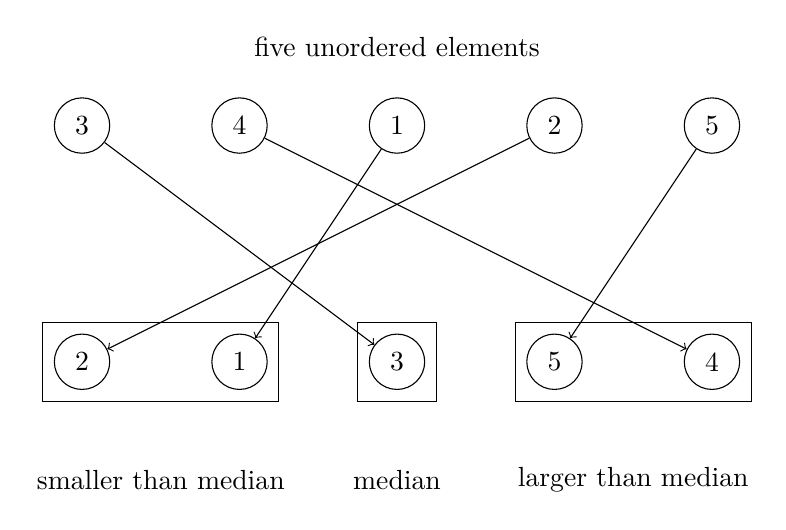
\begin{tikzpicture}

\node [shape=circle, draw=black, minimum size=2em] (v1) at (-3,1.5) {3};
\node [shape=circle, draw=black, minimum size=2em] (v3) at (-1,1.5) {4};
\node [shape=circle, draw=black, minimum size=2em] (v5) at (1,1.5) {1};
\node [shape=circle, draw=black, minimum size=2em] (v7) at (3,1.5) {2};
\node [shape=circle, draw=black, minimum size=2em] (v9) at (5,1.5) {5};
\node [shape=circle, draw=black, minimum size=2em] (v8) at (-3,-1.5) {2};
\node [shape=circle, draw=black, minimum size=2em] (v6) at (-1,-1.5) {1};
\node [shape=circle, draw=black, minimum size=2em] (v2) at (1,-1.5) {3};
\node [shape=circle, draw=black, minimum size=2em] (v10) at (3,-1.5) {5};
\node [shape=circle, draw=black, minimum size=2em] (v4) at (5,-1.5) {4};
\draw [->] (v1) edge (v2);
\draw [->] (v3) edge (v4);
\draw [->] (v5) edge (v6);
\draw [->] (v7) edge (v8);
\draw [->] (v9) edge (v10);
\node at (1,-3) {median};
\node at (-2,-3) {smaller than median};
\node at (4,-3) {larger than median};
\draw [->] (-3.5,-1) rectangle (-0.5,-2);
\draw [->] (2.5,-1) rectangle (5.5,-2);
\draw [->] (0.5,-1) rectangle (1.5,-2);
\node at (1,2.5) {five unordered elements};
\end{tikzpicture}
\end{center}
\caption{Median of 5}
\label{fig:median-of-5}
\end{figure}

\begin{lstlisting}[caption={Median of 5},label={lst:median:medofmeds},emph={M,median,by,medians,of}]
M5 : Set a -> bNat -> Set a
M5 A l = Indexed A l × Indexed A l -- the two smaller elements
       × Indexed A l               -- the median
       × Indexed A l × Indexed A l -- the two larger elements

median5-by :  (X -> A)
           -> X -> X -> X -> X -> X
           -> DecTree A (M5 X 5) 7


data Medians-Of-5 (A : Set a) (l : bNat) : Set a where
    medians :  Vec (M5 A l) \lfloor l /5\rfloor
            -> Vec (Indexed A l) (l % 5)
            -> Medians-Of-5 A l

_:::_ : M5 A 5 -> Medians-Of-5 A l -> Medians-Of-5 A (5 + l)


medians-of-5-by :  (X -> A) -> Vec X l
                -> DecTree A (Medians-Of-5 X l) (2 * l)
medians-of-5-by _ [] =
        return $ medians [] []
medians-of-5-by _ (a :: []) =
        delay 2 $
        return $ medians [] [ index f0 a ]
medians-of-5-by _ (a :: b :: []) =
        delay 4 $
        return $ medians [] $  (index f0 a)
                            :: [ index f1 b ]
medians-of-5-by _ (a :: b :: c :: []) =
        delay 6 $
        return $ medians [] $  (index f0 a)
                            :: (index f1 b)
                            :: [ index f2 c ]
medians-of-5-by _ (a :: b :: c :: d :: []) =
        delay 8 $
        return $ medians [] $  (index f0 a)
                            :: (index f1 b)
                            :: (index f2 c)
                            :: [ index f3 d ]
medians-of-5-by f (a :: b :: c :: d :: e :: xs) =
        let n = len xs in
        height-\equiv (sym $ *-distrib\^l-+ 2 5 n) $
        height-\equiv (cong (10 +_) $ +-identity\^r (2 * n)) $ do
        m5 <- delay 3 $ median5-by f a b c d e
        ms <- medians-of-5-by f xs
        return $ m5 ::: ms

\end{lstlisting}

The type \texttt{M5} (lines 1-4) over some type \texttt{A} is a 5-tuple of indexed elements of \texttt{A}, which represents the median of these five values alongside the smaller and larger elements.

The type \texttt{Medians-Of-5} (lines 11-14) represents the results of mapping this selection of the median of five elements over a full list. It contains a vector of the \texttt{M5} tuples that result from grouping the original data set into sets of five and selecting their respective median (line 12). Since the input data set's size may not be evenly divisible by five, we also store the remaining elements (line 13). The function \texttt{\_:::\_} prepends a median of five to the full result set, making sure to adjust the indices as required.

Finally, we implement the actual medians-of-5 function (lines 19ff.). We ignore the final remainder of the list if it is not divisible by 5 (see the cases in lines 23, 26, 30 and 35), and map our five-element median function over the rest (lines 45 and 46). Each step takes us slightly less than 10 units of time per five elements, and we bound this from above as two times the total size of the set.

Having done that, we can order these sets-of-5 \emph{themselves} by comparing their median values. By transitivity we know that in each set that is smaller than the median set, the leftmost three items are smaller than the median of the median values. This also holds symmetrically for the larger sets (see \autoref{fig:median-of-medians}).

\begin{figure}
\begin{center}
    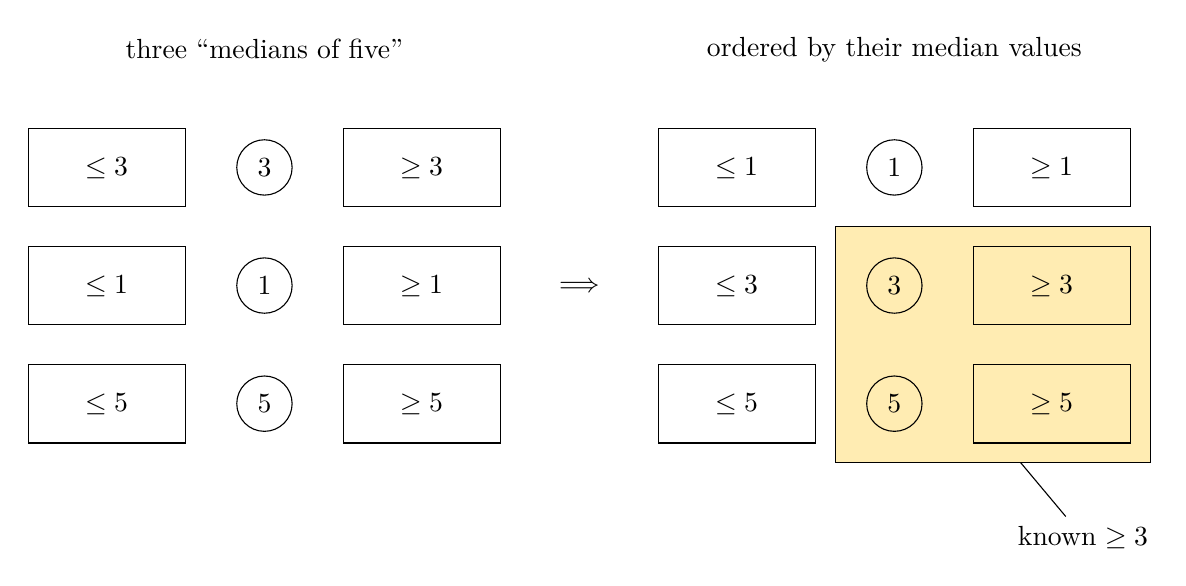
\begin{tikzpicture}
\definecolor{amber}{rgb}{1.0, 0.75, 0.0}

\draw [fill=amber, fill opacity=0.3] (7.25,3.75) rectangle (11.25,0.75);

\draw  (-3,5) rectangle (-1,4);
\node [shape=circle, draw=black, minimum size=2em] at (0,4.5) {3};
\draw  (1,5) rectangle (3,4);
\draw  (-3,3.5) rectangle (-1,2.5);
\draw  (1,3.5) rectangle (3,2.5);
\draw  (-3,2) rectangle (-1,1);
\draw  (1,2) rectangle (3,1);
\node [shape=circle, draw=black, minimum size=2em] at (0,3) {1};
\node [shape=circle, draw=black, minimum size=2em] at (0,1.5) {5};
\node at (0,6) {three ``medians of five"};
\node at (-2,4.5) {$\leq 3$};
\node at (2,4.5) {$\geq 3$};
\node at (-2,3) {$\leq 1$};
\node at (2,3) {$\geq 1$};
\node at (-2,1.5) {$\leq 5$};
\node at (2,1.5) {$\geq 5$};
\node at (4,3) {$\implies$};
\draw  (5,5) rectangle (7,4);
\draw  (9,5) rectangle (11,4);
\draw  (5,3.5) rectangle (7,2.5);
\draw  (9,3.5) rectangle (11,2.5);
\draw  (5,2) rectangle (7,1);
\draw  (9,2) rectangle (11,1);
\node [shape=circle, draw=black, minimum size=2em] at (8,4.5) {1};
\node [shape=circle, draw=black, minimum size=2em] at (8,3) {3};
\node [shape=circle, draw=black, minimum size=2em] at (8,1.5) {5};
\node at (8,6) {ordered by their median values};
\node at (6,4.5) {$\leq 1$};
\node at (10,4.5) {$\geq 1$};
\node at (6,3) {$\leq 3$};
\node at (10,3) {$\geq 3$};
\node at (6,1.5) {$\leq 5$};
\node at (10,1.5) {$\geq 5$};
\node (v1) at (10.4,-0.2) {known $\geq 3$};
\node (v2) at (9.5,0.875) {};
\draw  (v1) edge (v2);
\end{tikzpicture}
\end{center}
\caption{Median of medians}
\label{fig:median-of-medians}
\end{figure}

How do we select the median-of-medians? We fall back to the function we wanted to implement originally -- the median selection itself, now on the reduced data set of $\lfloor \frac n 5 \rfloor$.

\noindent\begin{minipage}{\linewidth}
\begin{lstlisting}[caption={Quasi-median and order statistic signatures},label={lst:median:quasimedian},emph={Quasi,Median,quasi,median,by,ordselect,Ordselect}]
Quasi-Median : Set a -> bNat -> Set a
Quasi-Median A l = Split A l
                   (\lambda x -> suc x \geq 3 * (l / 10))
                   (\lambda x -> suc x \geq 3 * (l / 10))

quasi-median-by :  let l = suc l-1 in
                   Acc _<_ l
                -> (X -> A)
                -> Vec X l
                -> DecTree A (Quasi-Median X l) (9 * l)

Ordselect : Set a -> (l : bNat) -> (i : Fin l) -> Set a
Ordselect A l i = Split A l
                  (_\equiv Data.Fin.tobNat i)
                  (_\equiv l Data.Fin.bNat-bNat (Data.Fin.raise 1 i))

ordselect-by :  let l = suc l-1 in
                Acc _<_ l
             -> (X -> A)
             -> (i : Fin l)
             -> (xs : Vec X l)
             -> DecTree A (Ordselect X l i) (35 * l)
\end{lstlisting}
\end{minipage}

Since our functions are mutually recursive, we have to pass an accessibility proof again. As with our sorting algorithms, we will show termination by way of the length of the vector.

Our elimination function will return a quasi-median (lines 1-4): A split that guarantees that 30\% (strictly speaking: $3 \cdot \lfloor \frac l {10}\rfloor$) of elements are smaller and greater than the selected median value. We furthermore guarantee that this is achievable in linear time with constant factor 9 (line 10).

In a similar vein, our ordselect (\emph{order statistic selection}) algorithm will return a split that guarantees that exactly $i$ elements are smaller than the $i$th order statistic and the remaining $l - i - 1$ elements are larger (lines 12-15). This too, is achievable in linear time, with constant factor 35.

\newpage
\begin{lstlisting}[caption={Quasi-median},label={lst:median:quasimedian}]
{- Cases for vectors of less than 5 elements omitted -}
quasi-median-by (Acc.acc more) f
                xs@(_ ∷ _ ∷ _ ∷ _ ∷ _ ∷ xss) =
    let l = suc l-1 in
    height-\equiv (sym $ *-distrib\^r-+ l 2 7) $
    height-\equiv (+-identity\^r (2 * l + 7 * l)) $
    height-\equiv (sym $ +-assoc (2 * l) (7 * l) 0 ) $
    do
        medians ms overflow <- medians-of-5-by f xs
        let ix = ix-half ms
        med-of-meds' <- delay-\leq (a*5*\lfloorn/5\rfloor\leqa*n 7 l) $
                        ordselect-by
                            (more \lfloor l /5\rfloor $ \lfloorl/5\rfloor<l _)
                            (f \circ m5-extract-value) ix ms
        let med-of-meds = simplify-med-split med-of-meds'
        return $ record
            { median = m5-extract-indexed $
                       Indexed.value $
                       Split.median med-of-meds
            ; smaller = small med-of-meds
            ; larger = large med-of-meds
            ; unknown = unk med-of-meds ++ overflow
            ; length-≡ = quasi-median-length-\equiv $ len xss
            ; bound-smaller = \leq-step $ \leq-step $ \leq-step \leq-refl
            ; bound-larger = a+a*n/10\geqa*\lceiln+5\rceil/10 3 (len xss)
            }
  where
    m5-extract-value    :  M5 A l -> A

    ix-half : Vec A (suc l-1) -> Fin (suc l-1)
    ix-half _ = frombNat< {m = \lfloor suc l-1 /2\rfloor} (n>0=>\lfloorn/2\rfloor<n _)

    simplify-med-split : let l = 5 + l-5 in
                   Ordselect (M5 A l) \lfloor l /5\rfloor (ix-half v)
                -> Split (M5 A l) \lfloor l /5\rfloor
                         (_\equiv \lfloor \lfloor l /5\rfloor /2\rfloor)
                         (_\equiv \lfloor \lfloor l-5 /5\rfloor /2\rfloor)

    small :  let l = 5 + l-5 in
             Split (M5 A l) \lfloor l /5\rfloor
                   (_\equiv \lfloor \lfloor l /5\rfloor /2\rfloor)
                   (_\equiv \lfloor \lfloor l-5 /5\rfloor /2\rfloor)
          -> Vec (Indexed A l) (2 + 3 * (l / 10))

    large :  let l = 5 + l-5 in
             Split (M5 A l) \lfloor l /5\rfloor
                   (_\equiv \lfloor \lfloor l /5\rfloor /2\rfloor)
                   (_\equiv \lfloor \lfloor l-5 /5\rfloor /2\rfloor)
          -> Vec (Indexed A l) (2 + 3 * (l-5 / 10))

    unk :  let l = 5 + l-5 in
           Split (M5 A l) \lfloor l /5\rfloor
                 (_\equiv \lfloor \lfloor l /5\rfloor /2\rfloor)
                 (_\equiv \lfloor \lfloor l-5 /5\rfloor /2\rfloor)
        -> Vec (Indexed A l) (2 * (l / 10) + 2 * (l-5 / 10))
\end{lstlisting}

We finally get to (one half of) the meat of our order statistic algorithm. For our quasi-median function, we first group our vector into ordered sets of five (line 9). We then select the \emph{actual} median of these sets, specifying that we want to order them by their middle value (line 11-14).

Selecting this median takes time $35 \cdot \lfloor \frac l 5 \rfloor$. We rewrite this in as a multiple of $l$ by showing that $35 \cdot \lfloor \frac l 5 \rfloor \leq 7 l$ (which, as most mathematical proofs in Agda is surprisingly non-trivial) in line 11.

Since the bounds for the size of the smaller and the larger section of quickselect's split are expressed in terms of the \texttt{Fin} number type, we reframe this in the \texttt{Nat} type by showing that the bounds are equivalent to $\lfloor \lfloor \frac l 5 \rfloor / 2 \rfloor$ and $\lfloor \lfloor \frac {l - 5} 5 \rfloor / 2 \rfloor$, respectively (line 15, using the function defined in line 33-37).

Finally, we extract the part that we are \emph{sure} is smaller than the selected median-of-medians (the ``top left" section in \autoref{fig:median-of-medians}) and similarly for the larger section (lines 20 and 21, respectively). Everything else, including the leftover elements that we could not group into sets of five, end up in the unknown block.

What remains is largely the mathematical proof burden to show that all of our bounds hold.

\begin{lstlisting}[caption={Quickselect (signature)},label={lst:median:quickselect},emph={ordselect,by}]
ordselect-by :  let l = suc l-1 in
                Acc _<_ l
             -> (X -> A)
             -> (i : Fin l)
             -> (xs : Vec X l)
             -> DecTree A (Ordselect X l i) (35 * l)

ordselect-by wf-acc f i xs with \leq-total (suc l-1) 8000
\end{lstlisting}

Finally, we come to an algorithmic sleight of hand: We can only prove that our quickselect bound holds when the length of the input is larger than 8000 (\autoref{lst:median:quickselect}, line 8): Whether we eliminate the larger or the smaller section of our quasi-median split, we can show that the length of the remainder (smaller and unknown or larger and unknown) is less than $7 \cdot \lfloor\frac l {10}\rfloor + 9$. To prove our desired bound of $35l$ for the whole of the algorithm, we need to show that recursing on this remainder (nominally $35\cdot(7 \cdot \lfloor\frac l {10} \rfloor + 9)$) is less than $25l$. However, the constant $+~9$ is getting in our way. We can rewrite the length of the vector as $70 \cdot \lfloor\frac l {100}\rfloor + 79$, which, under the assumption that $l > 800$, is less than $71 \cdot \lfloor\frac l {100}\rfloor$. With the constant so eliminated, we can eventually prove that the recursive call completes in time $25l$. The full proof is listed below.

However, for $l < 8000$, $\lceil \log_2 l \rceil$ is always below $13$ -- well within our bound! We therefore fall back to the sorting approach for this case, using our linear approach only where we can show it is within our (generous) bound.

\begin{lstlisting}[caption={Quickselect ($l \leq 8000$)},label={lst:median:quickselect:small},emph={ordselect,by,split,sorted,merge,sort}]
ordselect-by wf-acc f i xs with \leq-total (suc l-1) 8000
... | inj\_1 l\leq8000 = delay-\leq nlogn\leq35n $
                    split-sorted i <$> sorted
  where
    nlogn\leq35n : l * \lceillog\_2 l \rceil \leq 35 * l
    nlogn\leq35n = begin
        l * \lceillog\_2 l \rceil  \leq\langle *-mono\^r-\leq l $
                          n\leq8000=>\lceillog\_2n\rceil\leq35 l\leq8000 \rangle
        l * 35         \equiv\langle *-comm l 35 \rangle
        35 * l        \qed
    sorted = merge-sort-by (f \circ Indexed.value) $
             zipWith index (allFin l) xs
\end{lstlisting}

We index all the elements in the list, sort it and then split it at the specified location. Then we simply have to show that sorting the list is indeed faster than $35l$. For this proof (\texttt{nlogn$\leq$35n}, line 5-10) we introduce new notation: Equational reasoning. Equational reasoning relates two values (\texttt{l * $\lceil$log$_2$ l $\rceil$} in line 7 with \texttt{35 * l} in line 10) via a series of intermediate step. In our case, the relation will be $\leq$, specified by opening the module \texttt{Nat.Properties.$\leq$-Reasoning}.

The intermediate steps are related to each other by the functions \texttt{\_$\leq$$\langle$\_$\rangle$\_} and \texttt{\_$\equiv$$\langle$\_$\rangle$\_} which are effectively a way to write transitivity proofs in-line. The two functions are right-associative, thus we start analyzing this block of code from the end: the symbol $\qed$ is actually the function \texttt{\_$\qed$ : (x : $\mathbb N$) -> x $\leq$ x}, i.e. it just takes a value (in this case \texttt{35 * l}) and shows that it is related to itself. The function \texttt{\_$\leq$$\langle$\_$\rangle$\_} takes a value $x$ on the one side, a proof of $y \leq z$ on the other side and in between the angular brackets a proof that $x \leq y$ and yield a proof that $x \leq z$. The function \texttt{\_$\equiv$$\langle$\_$\rangle$\_} does the same, but in the brackets takes a proof of $x \equiv y$ instead. By chaining these methods, we can step by step construct a more complicated proof of one value being less or equal to another.


\begin{lstlisting}[caption={Quickselect ($l > 8000$)},label={lst:median:quickselect:large},emph={ordselect,by}]
ordselect-by wf-acc f i xs with \leq-total (suc l-1) 8000
... | inj\_2 l>8000 =
    let ibNat = tobNat i in
    height-\equiv (sym $ *-distrib\^r-+ l 9 26) $ do
        split <- quasi-median-by wf-acc f xs
        let l\_1 = Split.l\_1 split
        let l\_2 = Split.l\_2 split
        let l\_3 = Split.l\_3 split
        let median = Split.median split
        let unknown = Split.unknown split
        let l\_3\leql = \leq-trans
                     (m\leqn+m l\_3 (1 + l\_1 + l\_2))
                     (\leq-reflexive $ Split.length-\equiv split)
        unk-smaller , unk-larger by us+ul\equivl₃ <-
            delay-\leq l\_3\leql $
            split-pivot-by (f \circ Indexed.value) median unknown
        let smaller = Split.smaller split ++ unk-smaller
        let larger  = Split.larger  split ++ unk-larger
        let us\leql\_3 = \leq-trans
                      (m\leqm+n (len unk-smaller)
                             (len unk-larger))
                      (\leq-reflexive us+ul\equivl\_3)
        let ul\leql\_3 = \leq-trans
                      (m\leqn+m (len unk-larger)
                             (len unk-smaller))
                      (\leq-reflexive us+ul\equivl\_3)

        case ord ibNat (len smaller) of \lambda where
            (lt pf) -> delay-\leq (smallerRuntimeBound
                                    split
                                    (len unk-smaller)
                                    us\leql\_3) $
                       ordselect-lt
                           wf-acc f i
                           (Split.median split)
                           smaller larger
                           us+ul\equivl\_3
                           (Split.length-\equiv split)
                           pf
            (eq pf) -> delay-\leq z\leqn $ return $
                       ordselect-eq
                           i
                           (Split.median split)
                           smaller larger
                           us+ul\equivl\_3
                           (Split.length-\equiv split)
                           pf
            (gt pf) -> delay-\leq (largerRuntimeBound
                                    split
                                    (len unk-larger)
                                    ul\leql\_3) $
                       ordselect-gt
                           wf-acc f i
                           (Split.median split)
                           smaller larger
                           us+ul\equivl\_3
                           (Split.length-\equiv split)
                           pf
\end{lstlisting}

We first select the quasi median of the provided data in time $9l$ (line 5). We then further split the unknown data set into a larger and a smaller part with respect to this quasi median in time $l$ (line 14-16). Finally, we see how the length of the smaller data set compares to the index we are looking for (line 28): If the index is smaller, we just select with the same index from the smaller data set (case starting at line 29). If the index is equal, we simply return the selected quasi median (case starting at line 40). And if the index is larger, we subtract the size of the smaller data set from the index and use this to select from the larger data set (case starting in line 48).

As for the runtime, we show that selecting the median from the smaller or larger data set, which runs in time $35 \cdot \abs{\mathrm{\texttt{smaller}}}$ or $35 \cdot \abs{\mathrm{\texttt{larger}}}$ respectively, is faster than $25l$. Let us inspect this proof for the smaller case. The larger case follows by symmetry.

From the selection of the quasi-median, we know that

\[1 + \abs{\mathrm{\texttt{smaller}}_q} + \abs{\mathrm{\texttt{larger}}_q} + \abs{\mathrm{\texttt{unknown}}} = l\]

\vskip 1em
and

\[1 + \abs{\mathrm{\texttt{larger}}_q} \geq 3 \cdot \lfloor \frac l {10} \rfloor\]

where $\mathrm{\texttt{smaller}}_q$ and $\mathrm{\texttt{larger}}_q$ represent the Split sections returned by the quasi-median, in contrast with $\mathrm{\texttt{smaller}}_u$, which is the smaller part of the \texttt{unknown} section and $\mathrm{\texttt{smaller}}$, which is the concatenation of the former two.

We split the unknown set into a smaller and a larger set and add it to the smaller and larger set of the quasi median and thus have

\[\abs{\mathrm{\texttt{smaller}}} = \abs{\mathrm{\texttt{smaller}}_q} + \abs{\mathrm{\texttt{smaller}}_u}\]
\[\abs{\mathrm{\texttt{larger}}} = \abs{\mathrm{\texttt{larger}}_q} + \abs{\mathrm{\texttt{larger}}_u}\]
\[1 + \abs{\mathrm{\texttt{smaller}}} + \abs{\mathrm{\texttt{larger}}} = l\]

\vskip 1em
and by transitivity of $\leq$

\[1 + \abs{\mathrm{\texttt{larger}}} \geq 3 \cdot \lfloor \frac l {10} \rfloor.\]

\vskip 1em
Now we can show that

\begin{alignat*}{1}
    &\quad \abs{\mathrm{\texttt{smaller}}} \\
    =&\quad l - (1 + \abs{\mathrm{\texttt{larger}}}) \\
    \leq&\quad l - 3 \cdot \lfloor \frac l {10} \rfloor \\
    =&\quad l \bmod 10 + 10 \cdot \lfloor \frac l {10} \rfloor - 3 \cdot \lfloor \frac l {10} \rfloor \\
    =&\quad l \bmod 10 + 7 \cdot \lfloor \frac l {10} \rfloor \\
    \leq&\quad 7 \cdot \lfloor \frac l {10} \rfloor + 9.
\end{alignat*}

Under the assumption that $l \geq 8000$, we can further generalize this to

\begin{alignat*}{1}
    &\quad 7 \cdot \lfloor \frac l {10} \rfloor + 9 \\
    =&\quad 7 \cdot \lfloor \frac {10l} {100} \rfloor + 9 \\
    \leq&\quad 70 \cdot \lfloor \frac {l} {100} \rfloor + 79 \\
    \leq&\quad 70 \cdot \lfloor \frac {l} {100} \rfloor + \lfloor \frac {8000} {100} \rfloor \\
    \leq&\quad 70 \cdot \lfloor \frac {l} {100} \rfloor + \lfloor \frac {l} {100} \rfloor \\
    =&\quad 71 \cdot \lfloor \frac {l} {100} \rfloor.
\end{alignat*}

And thus selecting an order statistic from the smaller set takes time

\begin{alignat*}{1}
    &\quad 35 \cdot 71 \cdot \lfloor \frac {l} {100} \rfloor \\
    \leq&\quad 2500 \cdot \lfloor \frac {l} {100} \rfloor \\
    \leq&\quad 25 l.
\end{alignat*}

Knowing this, we can conclude that selecting the quasi median (time $9l$), splitting the unknown section (time $l$) and recursing on the appropriate smaller section (time $25l$) together takes total time $35l$, which is exactly the bound we wanted to show.
    % !TeX root = ../main.tex
% !TeX spellcheck = en_US

\chapter{Amortized Analysis}
\label{ch:amortized-analysis}
After having talked about deterministic worst-case bounds, let us now turn towards amortized analysis. Originally introduced in 1985 by Tarjan \cite{tarjan:1985:amortizedcc}, amortized analysis considers aggregate sequences of operations (starting from some initial element). This accounts for data structures where operations are usually fast, but occasionally slow. An example that may be familiar to a lot of people is C++'s \texttt{std::vector} and Java's \texttt{ArrayList}: Initially enough space for $n$ elements is allocated on the heap. This allows for $n$ insertions in constant time. On the $(n+1)$-th operation, twice as much space is allocated and the previous $n$ elements are copied over. This take $O(n)$ time, which if averaged with the previous operations results in \emph{amortized} constant time.

There are two main approaches to an amortized analysis: the banker's method and the potential method. They differ largely in how the calculate the cost for an individual operation. We will use the potential method in this thesis as it is more intuitive to implement.

\section{The Potential Method}
Intuitively, the potential method assigns to a data structure a measure of ``potential energy". An operation should generally increase this potential method when it takes little time. Conversely, an operation that takes a long time should use this accumulated potential energy to offset its cost. In the example above, an insert operation while there is still capacity would increase the potential by one. An insertion involving reallocating the list would reduce the potential by the number of elements in the list.

Let $S$ be a data structure. The potential method assigns a potential to every element $s \in S$ via a map $\varphi : S \rightarrow D$, where $D$ is some numerical domain. In this thesis, we will use $\mathbb N$ but using $\mathbb Q$ or $\mathbb R$ is equally possible. We ask two things of $\varphi$:

\newpage
\begin{itemize}
    \item The potential is never negative, $\varphi(s) \geq 0$.
    \item There is an ``initial" object $s_0$ from which the analysis starts (e.g. an empty list or an empty tree) and its potential is 0: $\varphi(s_0) = 0$.
\end{itemize}

Let $o_i$ be an operation that takes an object $s_i$ to an object $s_{i+1}$ and let $t(o_i)$ be the time it takes to compute $o_i$. Then the amortized time of this operation is

\[t_{am}(o_i) = t(o_i) - \varphi(s_i) + \varphi(s_{i+1}).\]
\vskip 1em

In other words, the amortized time is the actual time plus the \emph{change} in potential. For a sequence of operations $O = o_0, \ldots, o_n$ the total actual runtime is

\[T(O) = \sum_{i = 0}^n t(o_i)\]
\vskip 1em

and the total amortized runtime is

\begin{align*}
T_{am}(O) &= \sum_{i = 0}^n t_{am}(o_i) \\
&= \sum_{i = 0}^n t(o_i) - \varphi(s_i) + \varphi(s_{i+1}).
\end{align*}

Since this is a telescoping sum, we can simplify it by eliminating the intermediate potentials. Rewritten, it becomes

\[T_{am}(O) = \left(\sum_{i = 0}^n t(o_i)\right) - \varphi(s_0) + \varphi(s_{n+1}).\]
\vskip 1em

Since $\varphi(s_0) = 0$, this further reduces to

\[T_{am}(O) = T(O) + \varphi(s_{n+1})\]
\vskip 1em

and since potentials are always positive, the amortized runtime is an upper bound on the actual runtime.

\section{Ephemeral and Persistent Models of Computation}
In addition to the banker's and the potential method, amortized analysis also distinguishes two models of computation: The ephemeral and the persistent model. In the ephemeral model, objects can be used at most once. If they are used as input to an operation, they are replaced by the result. In the persistent model, previous states of the data structure remain accessible and can be reused as input to operations.

Going back to our vector example, in an ephemeral computing model, a list that has no remaining capacity can be inserted into only once. In a persistent model, the same list could be copied several times in this state, resulting in multiple high-cost operations. Clearly our analysis from above does not hold up in this case. In the PhD thesis of Okasaki \cite{okasaki:1998:purelyfunctionaldatastructures}, he has investigated the challenges of a persistent amortized analysis. For simplicity's sake, we will restrict ourselves to the ephemeral model of computation.

\section{Data Structures for an Amortized Analysis}
We introduce two datatypes: A record that defines the potential for a given type (\autoref{lst:amortized:framework:potential}) and a type to construct an amortized computation (\autoref{lst:amortized:framework:computation}).

\begin{lstlisting}[caption={Record defining the potential for a type A},label={lst:amortized:framework:potential},emph={Amortized,initial,potential,init}]
record Amortized (A : I -> Set a) : Set (a l\lub i) where
    field
        {i\_0} : I
        initial : A i\_0
        potential : {i : I} -> A i -> bNat
        init\equiv0 : potential initial \equiv 0
\end{lstlisting}

The potential defining record contains three fields of note: The definition of the potential function itself, the initial element of the data type and a proof that the potential of the initial object is in fact zero.

The datatype \texttt{Am} on the other hand provides us with several building blocks to construct an amortized computation.

\begin{lstlisting}[caption={Building blocks of an amortized computation},label={lst:amortized:framework:computation},emph={Am,Amortized,base,init,comp,step,bind,map,initial,DecTree}]
data Am (am : Amortized A) (C : Set b)
        : Set (Level.suc (a Level.\lub i Level.\lub b)) where
    base :  (x : A (Amortized.i\_0 am))
         -> {x \equiv Amortized.initial am}
         -> Am am C
    step :  {next : A i -> I}
            {time : A i -> bNat}
         -> Am am C
         -> ((x : A i) -> DecTree C (A $ next x) (time x))
         -> Am am C
    init-comp :  {B : Set a}
                 {time : bNat}
              -> DecTree C B time
              -> (B -> Am am C)
              -> Am am C
    am-bind :  {J : Set i}
               {B : J -> Set a}
               {am' : Amortized B}
            -> Am am' C
            -> (B j -> Am am C)
            -> Am am C
    am-map :  {J : Set i}
              {B : J -> Set a}
              {am' : Amortized B}
              {imap : B j -> I}
           -> (f : (x : B j) -> A $ imap x)
           -> {map-is-pot-invariant :
                   (x : B j)
                   ->   Amortized.potential am' x
                      \equiv Amortized.potential am (f x)}
           -> Am am' C
           -> Am am  C
\end{lstlisting}

The simplest here is \texttt{base} (line 3), which just contains the initial element and thus forms the base of the amortized computation. It is followed by \texttt{step} (line 6) which allows us to compose computations: Given an amortized computation, and a deterministic next step, the result is again an amortized computation.

Three additional constructors allow us to be more flexible in our handling of amortized computations. First, \texttt{init-comp} (line 11) allows us to follow a deterministic computation with an amortized one. Second, \texttt{am-bind} (line 16) allows us to take an amortized computation in one type and chain it into an amortized computation of a second type. Lastly, \texttt{am-map} (line 22) allows us to transform an amortized computation of one type entirely into one of another type, as long as we can prove that the potential for both is invariant under the transformation.

\subsection{A Note on Indexed Types}
An observant reader might notice that we use specifically indexed types. Why is that?

Consider the case of Agda's \texttt{Vec (A : Set) : $\mathbb N$ -> Set}. This is a \emph{family} of indexed types and \texttt{Vec A 0} and \texttt{Vec A 1} are distinct types. That means if we used simple types in our definition of \texttt{Amortized}, we'd need separate instances of it for all vectors of different lengths -- including distinct minimum elements.

Instead we allow for a family of indexed type with one parameter. For example, this allows us to generalize over vectors of arbitrary length for some fixed type, but not over vectors of arbitrary lengths and arbitrary types. Finding a way to be generic in the number of parameters to our family of indexed types would have been ideal, but we were not able to find such a method within the time constraints of this thesis. Allais (\cite{allais:2019:polymorphic-nary-functions}) had a promising approach that we were unable to evaluate before the deadline. Instead, as a proof of concept for this thesis, we special cased our framework to indexed families with one and with two parameters.

\section{Proof of Correctness}
We can now define a measure of the amortized runtime and show that it is indeed an upper bound on the actual runtime. We first define an evaluation function for an amortized computation:

\begin{lstlisting}[caption={Evaluating amortized computations},label={lst:amortized:framework:eval},emph={am,index,eval}]
am-index : Am am Compare -> I
am-eval :  {{_ : Leq C}}
        -> (v : Am am Compare)
        -> A (am-index v)
am-eval (base v)               = v
am-eval (step      val  trans) = reduce $ trans $ am-eval val
am-eval (am-map    f    val)   = f (am-eval val)
am-eval (am-bind   val  trans) = am-eval (trans $ am-eval val)
am-eval (init-comp comp trans) = am-eval (trans $ reduce comp)
\end{lstlisting}

The potential of a computation is then simply the potential of the result of the computation:

\begin{lstlisting}[caption={Potential of a computation},label={lst:amortized:framework:pot},emph={am,potential}]
am-potential : Am am Compare -> bNat
am-potential {am = am} v = Amortized.potential am $ am-eval v
\end{lstlisting}

The actual time of a computation is the sum of the worst-case guarantees of all individual steps:

\begin{lstlisting}[caption={Actual time},label={lst:amortized:framework:actualtime},emph={dtime,full}]
dtime-full : Am am Compare -> bNat
dtime-full (base val) = 0
dtime-full (step {_} {time} inner _) =
                    dtime-full inner
                    + time $ am-eval val
dtime-full (am-map _ val) = dtime-full val
dtime-full (am-bind val trans) =
                    dtime-full val
                    + dtime-full (trans $ am-eval val)
dtime-full (init-comp {_} {time} comp trans) =
                    time
                    + dtime-full (trans $ reduce comp)
\end{lstlisting}

The amortized time costs are defined as above, actual time less previous potential plus new potential for a computational step and just the deterministic time for an initial computation:
\begin{lstlisting}[caption={Amortized time},label={lst:amortized:framework:amortizedtime},emph={dtime,atime,step,full}]
atime-step : Am am Compare -> \bZ
atime-step (base val) = 0\bZ
atime-step (am-map _ _) = 0\bZ
atime-step (am-bind _ _) = 0\bZ
atime-step (init-comp {_} {time} _ _) = + time
atime-step v@(step val transform) = dtime-step v
                                    \ominus   pot-before
                                    \bZ.+ pot-after
    where
        val-before = am-eval val
        val-after = reduce $ transform $ val-before
        pot-before = Amortized.potential am $ val-before
        pot-after = Amortized.potential am val-after

atime-full : Am am Compare -> \bZ
atime-full (base val) = 0\bZ
atime-full (am-map _ val) = atime-full val
atime-full v@(step val _) =
                        atime-full val
                        \bZ.+ atime-step v
atime-full v@(init-comp comp trans) =
                        atime-step v
                        \bZ.+ atime-full (trans $ reduce comp)
atime-full (am-bind val trans) =
                        atime-full val
                        \bZ.+ atime-full (trans $ am-eval val)
\end{lstlisting}

All of this allows us to finally prove the central theorem of amortized runtime, that $T_{am}(O) \geq T(O) + \varphi(s_{n+1})$. The body of the proof is too long to print here and we refer the interested reader to the repository mentioned in \autoref{ch:layoftheland}.

\begin{lstlisting}[caption={Theorem: Amortized time is an upper bound on actual time},emph={atime,dtime,pot,full,potential}]
atime\geqdtime :  (v : Am am Compare)
               -> atime-full v
                  \bZ.\geq + (dtime-full v + am-potential v)
\end{lstlisting}
    % !TeX root = ../main.tex
% !TeX spellcheck = en_US

\chapter{Case Study: Binomial Heaps}
\label{ch:casestudyamortized}
As an example of how to use the framework we developed in the last chapter, let us take a look at binomial heaps. A heap is a data structure designed for quick access (and usually removal) of a minimum element. Use cases include, among other things, priority queues and sorting algorithms. Binomial heaps in particular were originally invented by Vuillemin \cite{vuillemin:1978:binheaps} and are special in that they combine a low-complexity implementation with reasonably fast operations, in particular computing the union of two heaps in logarithmic time.

\section{Theoretical Background}
First, we need to define binomial \emph{trees}. Binomial trees are already heaps in their own right, but with one notable restriction: The size of each tree is always a power of two. The logarithm of the size of a tree is called its rank.

A rank zero tree is just a single node:

\begin{figure}[h]
\begin{center}
    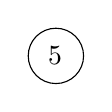
\begin{tikzpicture}

\node [shape = circle, minimum size = 2em, draw=black] at (0,0) {$5$};
\end{tikzpicture}
\end{center}
\caption{Binomial tree of rank 0}
\label{fig:binomial:rank0}
\end{figure}

A rank $n$ binomial tree is a root node with $n$ children: the first a rank $n-1$ tree, the second a rank $n-2$ child and so on. The value of each child node must be larger than that of the root node (\autoref{fig:binomial:rankn}).

\begin{figure}[h]
\begin{center}
    \begin{tikzpicture}

\node [shape=circle, minimum size = 2em, draw=black] (v1) at (0,0) {$3$};
\node [shape=circle, minimum size = 2em, draw=black] (v2) at (0,-1.5) {$6$};
\draw  (v1) edge (v2);
\node at (0,1) {Rank 1};
\node at (4.5,1) {Rank 2};
\node [shape=circle, minimum size = 2em, draw=black] (v3) at (4.5,0) {$2$};
\node [shape=circle, minimum size = 2em, draw=black] (v6) at (4.5,-1.5) {$5$};
\node [shape=circle, minimum size = 2em, draw=black] (v4) at (3,-1.5) {$4$};
\node [shape=circle, minimum size = 2em, draw=black] (v5) at (3,-3) {$7$};
\draw  (v3) edge (v4);
\draw  (v4) edge (v5);
\draw  (v3) edge (v6);
\node [shape=circle, minimum size = 2em, draw=black] (v7) at (11.5,0) {$3$};
\node [shape=circle, minimum size = 2em, draw=black] (v8) at (11.5,-1.5) {$9$};
\node [shape=circle, minimum size = 2em, draw=black] (v9) at (10,-1.5) {$6$};
\node [shape=circle, minimum size = 2em, draw=black] (v11) at (8.5,-1.5) {$7$};
\node [shape=circle, minimum size = 2em, draw=black] (v10) at (10,-3) {$7$};
\node [shape=circle, minimum size = 2em, draw=black] (v12) at (8.5,-3) {$9$};
\node [shape=circle, minimum size = 2em, draw=black] (v13) at (7,-3) {$9$};
\node [shape=circle, minimum size = 2em, draw=black] (v14) at (7,-4.5) {$9$};
\draw  (v7) edge (v8);
\draw  (v7) edge (v9);
\draw  (v9) edge (v10);
\draw  (v7) edge (v11);
\draw  (v11) edge (v12);
\draw  (v11) edge (v13);
\draw  (v13) edge (v14);
\node at (11.5,1) {Rank 3};
\end{tikzpicture}
\end{center}
\caption{Binomial trees of higher ranks}
\label{fig:binomial:rankn}
\end{figure}

We can join (or link, or merge) two trees of the same rank quickly by comparing their root nodes. The tree with the larger root becomes a child of the tree with the smaller one, increasing the rank of the new tree by one (\autoref{fig:binomial:merge}).

\begin{figure}[h]
\begin{center}
    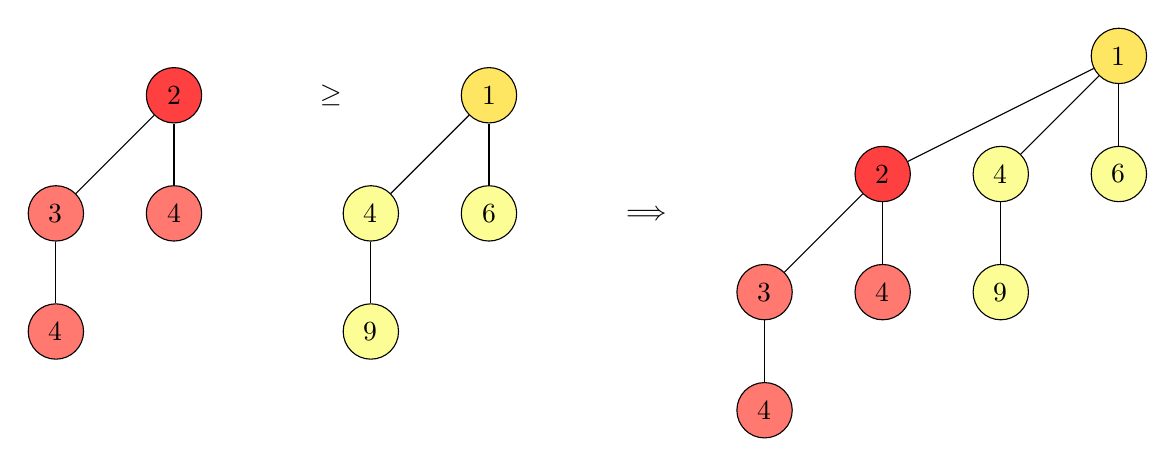
\begin{tikzpicture}
\definecolor{pastel-red}{HTML}{FF7971}
\definecolor{pastel-yellow}{HTML}{FDFD96}
\definecolor{sat-yellow}{HTML}{FFE662}
\definecolor{sat-red}{HTML}{FF4040}

\node [shape = circle, minimum size = 2em, draw = black, fill = sat-red] (v1) at (0,0) {$2$};
\node [shape = circle, minimum size = 2em, draw = black, fill = pastel-red] (v2) at (0,-1.5) {$4$};
\node [shape = circle, minimum size = 2em, draw = black, fill = pastel-red] (v3) at (-1.5,-1.5) {$3$};
\node [shape = circle, minimum size = 2em, draw = black, fill = pastel-red] (v4) at (-1.5,-3) {$4$};
\node [shape = circle, minimum size = 2em, draw = black, fill = sat-yellow] (v5) at (4,0) {$1$};
\node [shape = circle, minimum size = 2em, draw = black, fill = pastel-yellow] (v6) at (4,-1.5) {$6$};
\node [shape = circle, minimum size = 2em, draw = black, fill = pastel-yellow] (v7) at (2.5,-1.5) {$4$};
\node [shape = circle, minimum size = 2em, draw = black, fill = pastel-yellow] (v8) at (2.5,-3) {$9$};
\draw  (v1) edge (v2);
\draw  (v1) edge (v3);
\draw  (v3) edge (v4);
\draw  (v5) edge (v6);
\draw  (v5) edge (v7);
\draw  (v7) edge (v8);
\node at (2,0) {$\geq$};
\node at (6,-1.5) {$\implies$};


\node [shape = circle, minimum size = 2em, draw = black, fill = sat-red] (v21) at (9,-1) {$2$};
\node [shape = circle, minimum size = 2em, draw = black, fill = pastel-red] (v22) at (9,-2.5) {$4$};
\node [shape = circle, minimum size = 2em, draw = black, fill = pastel-red] (v23) at (7.5,-2.5) {$3$};
\node [shape = circle, minimum size = 2em, draw = black, fill = pastel-red] (v24) at (7.5,-4) {$4$};
\node [shape = circle, minimum size = 2em, draw = black, fill = sat-yellow] (v25) at (12,0.5) {$1$};
\node [shape = circle, minimum size = 2em, draw = black, fill = pastel-yellow] (v26) at (12,-1) {$6$};
\node [shape = circle, minimum size = 2em, draw = black, fill = pastel-yellow] (v27) at (10.5,-1) {$4$};
\node [shape = circle, minimum size = 2em, draw = black, fill = pastel-yellow] (v28) at (10.5,-2.5) {$9$};
\draw  (v25) edge (v26);
\draw  (v25) edge (v27);
\draw  (v27) edge (v28);
\draw  (v25) edge (v21);
\draw  (v21) edge (v22);
\draw  (v21) edge (v23);
\draw  (v24) edge (v23);
\end{tikzpicture}
\end{center}
\caption{Merging two binomial trees}
\label{fig:binomial:merge}
\end{figure}

Using these trees, we can now construct a binomial heap capable of storing any number of elements. We model a heap as a list of binomial trees of strictly increasing rank. A heap with $n$ elements has at most $1 + \lfloor \log_2 n \rfloor$ trees: The largest tree in this heap has rank $\lfloor \log_2 n \rfloor$ and then there can be only $\lfloor \log_2 n \rfloor$ trees with a smaller rank.

To find the minimum element, we iterate over all trees in the heap, finding the minimum among their root elements. Since there are only $\log n$ trees, this runs in $\mathcal O(\log n)$.

To insert an element into a heap, we create a rank zero tree containing just that element. Then we see if the heap contains a rank zero tree. If not, we can simply add the tree to the heap. Otherwise, we merge the two trees and repeat the process with the resulting rank one tree. This takes $k$ steps in total, where $k$ is the first rank for which no tree exists in the heap, $\mathcal O(\log n)$ in the worst case. However, we can show that the amortized runtime of an insert is constant:

Let $h$ be a heap. We define $\varphi(h)$ as the number of trees in the heap. Let

\[h' = insert(x, h)\]
\vskip 1em

be the result of inserting an element $x$ into $h$ and $k$ the minimum rank for which $h$ does not contain a tree. Then

\[t(insert(x, h)) = k\]
\vskip 1em

and

\[t_{am}(insert(x, h)) = k - \varphi(h) + \varphi(insert(x, h)).\]
\vskip 1em

Observe that the first $k$ trees of $h$ are removed after insertion because they are merged with the new tree. Instead, a new tree of rank $k$ is added. This means that $\varphi(insert(x, h)) = \varphi(h) - k + 1$ and thus $t_{am}(insert(x, h)) = 1$. A sequence of $n$ insert operations on an empty tree therefore has total amortized runtime $n$, so a single operation runs in amortized time $\mathcal O(1)$.

We can also merge two heaps in $\mathcal O(\log \max(k_1, k_2))$ where $k_1$ and $k_2$ are the number of elements in either heap. Starting at rank zero, we check if the two heaps both contain a tree of that rank. If not, we simply copy the tree of the heap that does, or leave the slot empty if neither does. If both heaps contain a tree, we join the two and insert the result into the result heap at rank one. We then continue with the next rank. Observe that after merging up to and including rank $(n-1)$, we will have filled at most the rank $n$ slot of the result heap. If both trees contain a rank $n$ tree, we merge them into a rank $(n+1)$ tree and insert that. If only one heap does and the result also contains a rank $n$ tree from the previous merge step, we merge these two into a rank $(n+1)$ tree. By our invariant, this slot is still free. Put the merged rank $(n+1)$ tree thus maintains that invariant as we have just completed the merge up to tank $n$. Otherwise, if only one of the two heaps and not the result contains a rank $n$ tree, we insert that single tree into the result. Each individual merge step runs in time $\mathcal O(1)$, and therefore the full merge runs in time $\mathcal O(\log \max(k_1, k_2))$.

Finally, we can remove the minimum element from a heap in time $\mathcal O(\log n)$. We find the minimum element as before. This time, we remove this tree in its entirety from the heap. This still leaves us with a valid heap. Since the child elements of a tree of rank $n$ are trees of rank $0$ to $n-1$, we can consider these child elements a heap in their own right (recall that we model heaps as lists of trees with distinct ranks). We therefore merge the child elements of the removed tree back into the main heap. Finding the minimum tree takes time $\mathcal O(\log n)$. Both the heap after removing a full tree and the heap formed by the children have a size less than the original heap. The merge therefore completes in time $\mathcal O(\log n)$ as well.

\section{Implementation}
With the theory out of the way, let us now consider how to implement this in our framework for amortized analysis.

A descending list of length $l$ of a type indexed by the natural numbers is a list where the first element is indexed by $l$, the second by $l-1$ and so on up to the $l$-th element indexed by zero (\autoref{lst:binomial:tree}, lines 1-3). A binomial tree over a set $A$ is then either a leaf of rank zero, containing just a single element of $A$ (line 5), or a node of rank $l+1$ containing an element of $A$ and a descending list of binomial trees of length $l$ (lines 7-9)

\begin{lstlisting}[caption={Definition of a binomial tree},label={lst:binomial:tree},emph={DescList,BinomialTree,Leaf,Node}]
data DescList (A : bNat -> Set a) : bNat -> Set a where
    D[_] : A 0 -> DescList A 0
    _D::_ : A (suc l) -> DescList A l -> DescList A (suc l)

data BinomialTree (A : Set a) : bNat -> Set a where
    Leaf : A -> BinomialTree A 0
    Node :  A
         -> DescList (BinomialTree A) l
         -> BinomialTree A (suc l)

tSize : BinomialTree A l -> bNat
tSize {l = l} _ = 2 ^ l

tVal : BinomialTree A l -> A
tVal (Leaf x) = x
tVal (Node x _) = x
\end{lstlisting}

We can merge two trees of equal rank in constant time:

\begin{lstlisting}[caption={Merging two trees},label={lst:binomial:link},emph={link,Leaf,Node,if,then,else}]
link :  BinomialTree A l
     -> BinomialTree A l
     -> DecTree A (BinomialTree A (suc l)) 1
link (Leaf l) (Leaf r) = if l ≤? r
                         then return (Node l $ D[ Leaf r ])
                         else return (Node r $ D[ Leaf l ])
link l@(Node x xs) r@(Node y ys) =
                         if x ≤? y
                         then return (Node x $ r D:: xs)
                         else return (Node y $ l D:: ys)
\end{lstlisting}

A heap is represented as a contiguous list running from some minimum rank $l$ to rank $l + k$. At every position there is either a binomial tree of that rank or an empty slot. Slots below $l$ or above $l + k$ are implicitly left empty. The list is indexed by two natural numbers: The minimum rank, $l$, and the total number of elements stores in the heap. The number of entries of such a list is the number of trees (or: non-empty slots) contained in it.

An empty heap can have any minimum rank and contains an element (\autoref{lst:binomial:heap}, line 2). An empty entry extends a heap with minimum rank $l+1$ to one with minimum rank $l$ (lines 3-4). Finally, a filled entry combines a tree of rank $l$ with a heap with minimum rank $l+1$ and $acc$ items into a heap of minimum rank $l$ and $2^l + acc$ items (lines 5-9).

\begin{lstlisting}[caption={Definition of a binomial heap},label={lst:binomial:heap},emph={SparseTreeList,empty,entry,BinomialTree,entries}]
data SparseTreeList (A : Set a) : bNat -> bNat -> Set a where
    []        :  SparseTreeList A l 0
    empty::   :  SparseTreeList A (suc l) acc
              -> SparseTreeList A l acc
    entry_::_ :  {l acc acc' : bNat}
              -> {acc'\equiv2^l+acc : acc' \equiv 2 ^ l + acc}
              -> BinomialTree A l
              -> SparseTreeList A (suc l) acc
              -> SparseTreeList A l acc'


ts-acc : SparseTreeList A l acc -> bNat
ts-acc {acc = acc} _ = acc

entries : SparseTreeList A l acc -> bNat
entries [] = 0
entries (empty:: ts) = entries ts
entries (entry _ :: ts) = 1 + entries ts
\end{lstlisting}

For completeness' sake we prove that the number of entries of a heap is bounded by the logarithm of total elements stored. As usual with long purely mathematical proofs we omit the proof body. The signature can be found in \autoref{lst:binomial:bounded}.

\begin{lstlisting}[caption={The length of a heap is bounded},label={lst:binomial:bounded},emph={SparseTreeList, entries}]
len\leq\lfloorlog\_2acc\rfloor :  (ts : SparseTreeList A l acc)
              -> entries ts \leq 1+\lfloorlog\_2 acc \rfloor
\end{lstlisting}

We can now provide \texttt{Amortized} declarations for a heap. We have two: One for heaps over a type $A$ and one for heaps over a type $A$ with minimum rank $0$.

\begin{lstlisting}[caption={Amortized declaration},label={lst:binomial:amortized},emph={tlist,amortized,Amortized}]
tlist-amortized0 :  (A : Set a)
                 -> Amortized (SparseTreeList A 0)
Amortized.i\_0        (tlist-amortized0 A) = 0
Amortized.initial   (tlist-amortized0 A) = []
Amortized.potential (tlist-amortized0 A) = entries
Amortized.init\equiv0    (tlist-amortized0 A) = refl

tlist-amortized' :  (A : Set a)
                 -> Amortized1 (SparseTreeList A)
Amortized1.i\_0        (tlist-amortized' A)   = 0
Amortized1.initial   (tlist-amortized' A) l = []
Amortized1.potential (tlist-amortized' A)   = entries
Amortized1.init\equiv0    (tlist-amortized' A) l =
        \leq-antisym (len\leq\lfloorlog\_2acc\rfloor
            (Amortized1.initial (tlist-amortized' A) l))
        z\leqn
\end{lstlisting}

We implement insertion into a heap where the minimum rank of the heap matches the rank of the inserted tree. This is sufficient for insertion of single elements into a heap with minimum rank zero.

If the heap is empty or the rank $n$ slot is free, this means simply slotting the tree at the right position (\autoref{lst:binomial:insert}, lines 6-7). Otherwise, we merge the new and the present tree (line 9) and insert them in the remainder of the heap (line 12).

\begin{lstlisting}[caption={Inserting into a heap},label={lst:binomial:insert},emph={BinomialTree,SparseTreeList,insertTList,empty,entry}]
insertTList\equiv :  BinomialTree A l
             -> (ts : SparseTreeList A l acc)
             -> DecTree A
                  (SparseTreeList A l (2 ^ l + acc))
                  (leadingEntries ts)
insertTList\equiv t [] = return $ entry t :: []
insertTList\equiv t (empty:: ts) = return $ entry t :: ts
insertTList\equiv t (entry t' :: ts) = do
    t-join <- link t t'
    tlist-dec-subst-acc
        (+-assoc (2 ^ l) (2 ^ l) acc') $
    empty:: <$> insertTList\equiv t-join ts
\end{lstlisting}

Now we can show that a single insertion's amortized runtime is constant. Recall that the amortized runtime is the actual runtime (leading non-empty entries in the tree) plus the change in potential (total non-empty entries).

For the empty heap and a heap with a leading empty entry, this is straightforward (\autoref{lst:binomial:constinsert}, lines 7-9).

In the non-empty case, we insert a tree $t$ into a heap $ts$, that is, a tree $x$ concatenated with a heap $ts'$ (line 10). We first use the fact that $leadingEntries(ts) - entries(ts)$ reduces to $leadingEntries(ts')-entries(ts')$ (line 11-12 contrasted with 17-18). We then show that the number of entries when inserting $t$ into $ts$ is the same as when inserting the linked tree $link(t, x)$ into $ts'$ (proof in lines 27ff., used in line 13 contrasted with lines 19-20). We can then show this rewritten runtime to be equal to 1 by recursing on $link(t, x)$ and $ts'$.

\begin{lstlisting}[caption={Insertion runs in constant time},label={lst:binomial:constinsert},emph={tlist,insert,pot,invariant,empty,entry,BinomialTree,SparseTreeList,leadingEntries,entries,insertTList}]
tlist-insert-pot-invariant :
              (t : BinomialTree A l)
           -> (ts : SparseTreeList A l acc)
           -> leadingEntries ts \ominus entries ts
              \bZ.+ entries (reduce $ insertTList\equiv t ts)
              \equiv + 1
tlist-insert-pot-invariant t [] = refl
tlist-insert-pot-invariant t (empty:: ts) =
            0-a+suca\equiv1 (entries ts)
tlist-insert-pot-invariant t ts@(entry x :: ts') = begin
      leadingEntries ts
    \ominus entries ts
    \bZ.+ entries (reduce $ insertTList\equiv t ts)

            \equiv\langle {- einsert -} \rangle

      leadingEntries ts'
    \ominus entries ts'
    \bZ.+ entries (reduce $
                 insertTList\equiv (reduce $ link t x) ts')

            \equiv\langle {- induction on (link t x), ts' -} \rangle

    + 1  \qed
  where
    einsert : entries (reduce $ insertTList\equiv t ts)
            \equiv entries (reduce $ insertTList\equiv
                                     (reduce $ link t x) ts')
    einsert = begin
        entries (reduce (insertTList\equiv t ts))

            \equiv\langle {- bind-elim -} \rangle

        entries (reduce (empty:: <$>
                         insertTList\equiv (reduce (link t x)) ts'))

            \equiv\langle {- apply-elim -} \rangle

        entries (reduce $ insertTList\equiv
                            (reduce $ link t x) ts')

            \qed

\end{lstlisting}

We can use this to show that performing $n$ insertions into an empty list runs in $\mathcal O(n)$. First, we define an amortized computation performing $n$ insertions from a vector (\autoref{lst:binomial:ins-in-linear-time}, lines 1-5). We then show that the total amortized runtime of this computation is exactly $n$ (line 9): Initially, we recurse on the first $n-1$ insertions (line 15 contrasted with line 22) and then apply the lemma from \autoref{lst:binomial:constinsert} to substitute the second term with 1 (line 22-24 contrasted with line 28).

\begin{lstlisting}[caption={$n$ inserts in linear time},label={lst:binomial:ins-in-linear-time},emph={tlist,insert,inserts,n,in,linear,time,insertTList,am,leadingEntries,potential}]
tlist-n-inserts : Vec A n -> Am (tlist-amortized0 A) A
tlist-n-inserts zero Vec.[] = lift
tlist-n-inserts (suc n) (x :: xs) = Am.step
                (tlist-n-inserts n xs)
                (\lambda ts -> insertTList\equiv (Leaf x) ts)

tlist-insert-in-linear-time :
                   (xs : Vec A n)
                -> atime-full (tlist-n-inserts xs) ≡ + n
tlist-insert-in-linear-time Vec.[] = refl
tlist-insert-in-linear-time (x :: xs) =
    let n-1-inserts = tlist-n-inserts xs in
    let n-inserts = tlist-n-inserts (x :: xs) in begin

        atime-full n-1-inserts
        \bZ.+ (leadingEntries (am-eval n-1-inserts)
             \ominus   am-potential n-1-inserts
             \bZ.+ am-potential n-inserts)

            \equiv\langle {- induction -} \rangle

        + n-1 \bZ.+ (leadingEntries (am-eval n-1-inserts)
                   \ominus   am-potential n-1-inserts
                   \bZ.+ am-potential n-inserts)

            \equiv\langle {- tlist-insert-pot-invariant -} \rangle

        + (n-1 + 1)  \qed
  where
    open ≡-Reasoning
\end{lstlisting}

In a similar vein, we can implement the remaining operations of a binomial heap: Merging two heaps, finding the minimum element and building on top of that, removing the minimum element from the heap. We list just there function signatures and omit the bodies for brevity's sake; the proof patterns used are similar to those used in \autoref{lst:binomial:constinsert} and \autoref{lst:binomial:ins-in-linear-time}. Interested readers may want to check the appendix, \autoref{sec:heap-additional} for the full code.

\begin{lstlisting}[caption={Remaining heap operations},label={lst:binomial:remaining},emph={SparseTreeList,tListMergeAm,merge,in,log,time,findMin,deleteMin}]
tListMergeAm :  (left : SparseTreeList A l acc)
             -> (right : SparseTreeList A l' acc')
             -> Am1 (tlist-amortized' A) A (l \lub l')

merge-in-log-time :  (left : SparseTreeList A l acc)
                  -> (right : SparseTreeList A l' acc')
                  -> atime-full1 (tListMergeAm left right) \
                     \bZ.\leq 2 * 1+\lfloorlog\_2 acc \lub acc' \rfloor

findMin :  SparseTreeList A l (suc acc)
        -> DecTree A A 1+\lfloorlog\_2 (suc acc) \rfloor

deleteMin :  (ts : SparseTreeList A l (suc acc))
          -> Am1 (tlist-amortized' A) A 0


deleteMin-in-log-time :  (ts : SparseTreeList A l (suc acc))
                      -> atime-full1 (deleteMin ts)
                         \bZ.\leq + 3 * 1+\lfloorlog\_2 suc acc \rfloor

\end{lstlisting}
    % !TeX root = ../main.tex
% !TeX spellcheck = en_US

\chapter{Conclusion}
In the Case Studies chapters, we have shown how to use the frameworks we have designed: examples of deterministic worst case bounds in \autoref{ch:casestudiesdeterministic} and amortized bounds in \autoref{ch:casestudyamortized}. These frameworks do carry overhead with them: During execution proof objects need to be constructed and the framework's wrapper objects need to be assembled and broken down again. Additionally, there is a non-negligible syntactic overhead due to the sheer volume of code required to proof properties in Agda. Nonetheless, as far as formal verification of runtime is concerned this is a win.

There are three main avenues to continue the work presented in this thesis: Firstly, extending the framework with additional transformations and proof functions that make working with it more seamless, especially with an eye towards easing the syntactic burden. An obvious candidate for this might be a redefinition of \texttt{\_>>=\_} similar to the redefinition of \texttt{\_*\_} provided in the module \texttt{Nat.Mul}. The former introduces a trailing $0$ in the run time bound when the final statement of a do-block is a \texttt{return}, the latter introduces a trailing $0$ when the first factor of a multiplication is a constant. These trailing zeroes need to be manually eliminated with \texttt{+-identity$^r$}.

The second avenue is reducing the run time overhead of the framework, for example by judicious use of proof elimination. Given the blurred line of compile- and run-time in dependently typed language, this goes hand in hand with increasing type checking responsiveness.

As a third major point, eliminating the need of special-cased implementations of \texttt{Amortized} and \texttt{Am} based on the number of parameters to the type would go a long way towards making this framework more usable.

Real-time and embedded systems are an obvious candidate for resource verification. However for the degree of accuracy needed for these systems we would need to descend an abstraction level from "number of comparisons" to a more direct representation of time elapsed. An added hurdle is of course that Haskell, and by extension Agda, are not usually first-choice languages for real-time systems. Developing an sound wall-clock framework with no or provably limited runtime overhead in a language suitable for embedded development might be the holy grail of this avenue of research.

Ours is not the first approach to analyzing time bounds. Nipkow in \cite{nipkow:2017:verified-root-balanced-trees} and Danielsson in \cite{danielsson:2008:time-complexity-analysis} have implemented similar time-tracking monads as we have, with the notable difference of relying on the programmer to track time spent correctly. Nipkow has also investigated amortized analyses in \cite{nipkow:2015:amortizedverified}, also relying on programmers manually specifying the time an operation needs to complete.

Time is not the only resource for which upper bounds are interesting. For example Brady and Hammond \cite{brady:2006:programsize} have tried to derive memory bounds by statically analyzing the size of data structures. Liqat et al. \cite{liqatetal:2013:energyconsumption} have investigated ways to analyze the power consumption of embedded software.



	\printbibliography

    \clearpage
    \pagenumbering{roman}
    \setcounter{page}{0}
    \part*{Appendices}

    \appendix
    \chapter{Extended Code Listings}
    \lstset{
        basicstyle=\footnotesize\ttfamily\color{solarized-default},
        breaklines=true,
        breakatwhitespace=true,
        numberstyle={\footnotesize\ttfamily\color{darkgray}},
    }
    \label{ch:extendedcodelistings}
    \section{Amortized Data Structures for Types with Two Indices}
\label{sec:atime1}
\begin{lstlisting}[caption={Amortized data structures and functions for data types with two indices},label={lst:appendix:atime1}]
record Amortized1 {A : Set a} {I : Set i} (P : A -> I -> Set b) : Set (a Level.\lub b Level.\lub i) where
    field
        {i\_0} : I
        initial : (a : A) -> P a i\_0
        potential : {a : A} {i : I} -> P a i -> bNat
        init\equiv0 : (a : A) -> potential (initial a) \equiv 0

data Am1 {A : Set a} {I : Set i} {P : A -> I -> Set b} (am : Amortized1 P) (C : Set c)
        : A -> Set (Level.suc (a Level.\lub i Level.\lub b Level.\lub c)) where
    base :  {a : A}
         -> (v : P a (Amortized1.i\_0 am))
         -> {v \equiv Amortized1.initial am a}
         -> Am1 am C a
    init-comp :  {B : Set b}
                 {time : bNat}
                 {a : A}
              -> DecTree C B time
              -> (B -> Am1 am C a)
              -> Am1 am C a
    step :  {nextA : A -> A}
            {nextI : {a : A} {i : I} -> P a i -> I}
            {time  : {a : A} {i : I} -> P a i -> bNat}
            {a : A}
         -> Am1 am C a
         -> ({i : I} -> (x : P a i) -> DecTree C (P (nextA a) (nextI x)) (time x))
         -> Am1 am C (nextA a)

lift1 : {P : M -> I -> Set a} {am : Amortized1 P} -> (m : M) -> Am1 am Compare m
lift1 {am = am} m = base (Amortized1.initial am m) {refl}

am1-index : {P : M -> I -> Set a} {am : Amortized1 P} {{_ : Leq Compare}} {m : M} -> Am1 am Compare m -> I
am1-eval : {P : M -> I -> Set a} {am : Amortized1 P} {m : M} -> {{_ : Leq Compare}} -> (v : Am1 am Compare m) -> P m (am1-index v)

am1-index {am = am} (base _) = Amortized1.i\_0 am
am1-index (step {nextI = nextI} val _) = nextI (am1-eval val)
am1-index (init-comp comp trans) = am1-index (trans $ reduce comp)

am1-eval (base v) = v
am1-eval (step val trans) = reduce $ trans $ am1-eval val
am1-eval (init-comp comp trans) = am1-eval $ trans $ reduce comp

am1-potential : {P : M -> I -> Set a} {am : Amortized1 P} {m : M} {{_ : Leq Compare}} -> Am1 am Compare m -> bNat
am1-potential {am = am} v = Amortized1.potential am $ am1-eval v

dtime-step1 : {P : M -> I -> Set a} {am : Amortized1 P} {m : M} {{_ : Leq Compare}} -> Am1 am Compare m -> bNat
dtime-step1 (base val) = 0
dtime-step1 (step {time = time} val trans) = time $ am1-eval val
dtime-step1 (init-comp {_} {time} _ _) = time

dtime-full1 : {P : M -> I -> Set a} {am : Amortized1 P} {m : M} {{_ : Leq Compare}} -> Am1 am Compare m -> bNat
dtime-full1 (base val) = 0
dtime-full1 outer@(step inner _) = dtime-full1 inner + dtime-step1 outer
dtime-full1 (init-comp {_} {time} comp trans) = time + dtime-full1 (trans $ reduce comp)


atime-step1 : {P : M -> I -> Set a} {am : Amortized1 P} {m : M} {{_ : Leq Compare}} -> Am1 am Compare m -> \bZ
atime-step1 (base val) = \bZ.0\bZ
atime-step1 (init-comp {_} {time} _ _) = + time
atime-step1 {am = am} v@(step val transform) = dtime-step1 v \ominus pot-before \bZ.+ (+ pot-after)
    where
        val-before = am1-eval val
        val-after = reduce $ transform $ val-before
        pot-before = Amortized1.potential am val-before
        pot-after = Amortized1.potential am val-after

atime-full1 : {P : M -> I -> Set a} {am : Amortized1 P} {m : M} {{_ : Leq Compare}} -> Am1 am Compare m -> \bZ
atime-full1 (base val) = \bZ.0\bZ
atime-full1 v@(init-comp comp trans) = atime-step1 v \bZ.+ atime-full1 (trans $ reduce comp)
atime-full1 v@(step val _) = atime-full1 val \bZ.+ atime-step1 v
\end{lstlisting}
    \newpage
\section{Amortized Time Bound On Actual Time}
\label{sec:atime-proof}
\begin{lstlisting}[caption={Amortized time bounds actual time from above},label={lst:appendix:atime-proof}]
atime\geqdtime : {am : Amortized A} -> {{_ : Leq Compare}} -> (v : Am am Compare) -> atime-full v \bZ.\geq + (dtime-full v + am-potential v)
atime\geqdtime {am = am} (base v {v\equivinit}) = \bZ.+\leq+ (\leq-reflexive $ trans (cong (Amortized.potential am) v\equivinit) (Amortized.init\equiv0 am))
atime\geqdtime v@(am-map f {map-pot-inv} val) = begin
        + (dtime-full val + am-potential v)          \equiv\langle cong (\lambda x -> + (dtime-full val + x)) $ sym $ map-pot-inv (am-eval val)  ⟩
        + (dtime-full val + am-potential val)        \leq\langle atime\geqdtime val \rangle
        atime-full val                               \qed
    where
        open \bZ-Props.\leq-Reasoning
atime\geqdtime v@(init-comp {_} {time} comp trans) = begin
        + (time + dtime-full (trans $ reduce comp) + am-potential v)     \equiv\langle cong (+_) $ +-assoc time _ _ \rangle
        + (time + (dtime-full (trans $ reduce comp) + am-potential v))   \leq\langle \bZ-Props.+-mono\^r-\leq (+ time) $ atime\geqdtime (trans $ reduce comp) \rangle
        + time \bZ.+ atime-full (trans $ reduce comp)                      \qed
    where
        open \bZ-Props.\leq-Reasoning
atime\geqdtime (am-bind val trans) = begin
        + (dtime-full val + dtime-full (trans $ am-eval val) + am-potential (trans $ am-eval val))
                    \equiv\langle cong (+_) $ +-assoc (dtime-full val) _ _ \rangle
        + (dtime-full val + (dtime-full (trans $ am-eval val) + am-potential (trans $ am-eval val)))
                    \leq\langle \bZ-Props.+-mono\^r-\leq (+ dtime-full val) $ atime\geqdtime (trans $ am-eval val) \rangle
        + dtime-full val \bZ.+ atime-full (trans $ am-eval val)
                    \leq\langle \bZ-Props.+-mono\^l-\leq (atime-full $ trans $ am-eval val) $ \bZ.+\leq+ $ m≤m+n (dtime-full val) (am-potential val) \rangle
        + (dtime-full val + am-potential val) \bZ.+ atime-full (trans $ am-eval val)
                    \leq\langle \bZ-Props.+-mono\^l-\leq _ $ atime\geqdtime val \rangle
        atime-full val \bZ.+ atime-full (trans $ am-eval val)
                    \qed
    where
        open \bZ-Props.\leq-Reasoning
atime\geqdtime v@(step val trans) = begin
        + (dtime-full val + dtime-step v + am-potential v)

                    \equiv\langle cong (\bZ._+ (+ am-potential v)) $ sym $ +-telescope (+ dtime-full val) (+ dtime-step v) (+ am-potential val) \rangle

        + (dtime-full val + am-potential val) \bZ.+ (+ dtime-step v \bZ.- + am-potential val) \bZ.+ + am-potential v

                    \equiv\langle cong (\lambda x -> + (dtime-full val + am-potential val) \bZ.+ x \bZ.+ + am-potential v) $ \bZ-Props.[+m]-[+n]≡m\ominusn (dtime-step v) (am-potential val) \rangle

        + (dtime-full val + am-potential val) \bZ.+ (dtime-step v \ominus am-potential val) \bZ.+ + am-potential v

                    \equiv\langle \bZ-Props.+-assoc (+ (dtime-full val + am-potential val)) (dtime-step v \ominus am-potential val) (+ am-potential v) \rangle

        + (dtime-full val + am-potential val) \bZ.+ (dtime-step v \ominus am-potential val \bZ.+ + am-potential v)

                    ≡⟨⟩

        + (dtime-full val + am-potential val) \bZ.+ atime-step v

                    \leq\langle \bZ-Props.+-mono\^l-\leq _ $ atime\geqdtime val \rangle

        atime-full val \bZ.+ atime-step v   \qed
    where
        open \bZ-Props.\leq-Reasoning
\end{lstlisting}
    \newpage
\section{Additional Heap Functions}
\label{sec:heap-additional}
\begin{lstlisting}[caption={Merging heaps},label={lst:appendix:heap:merge}]
tListMergeAm\equiv :  {l acc acc' : bNat}
              -> (left : SparseTreeList A l acc)
              -> (right : SparseTreeList A l acc')
              -> Am1 (tlist-amortized' A) A l
tListMergeAm\equiv {l = l} {acc' = acc'} [] right =
                Am1.step {nextA = const l} {nextI = const acc'} {time = const 0}
                (lift1 0) (\lambda _ -> return right)
tListMergeAm\equiv {l = l} {acc = acc} (empty:: left) [] =
                Am1.step {nextA = const l} {nextI = const acc} {time = const 0}
                (lift1 0) (\lambda _ -> return $ empty:: left)
tListMergeAm\equiv (empty:: left) (empty:: right) =
                Am1.step {nextA = pred} {nextI = ts-acc} {time = const 0}
                (tListMergeAm\equiv left right) (\lambda ts -> return $ empty:: ts)
tListMergeAm\equiv {l = l} (empty:: left) (entry x :: right) =
                Am1.step {nextA = pred} {nextI = \lambda ts -> 2 ^ l + ts-acc ts} {time = const 0}
                (tListMergeAm\equiv left right) (\lambda ts -> return $ entry_::_ {acc' = 2 ^ l + ts-acc ts} {acc'\equiv2^l+acc = refl} x ts)
tListMergeAm\equiv {l = l} {acc = acc} left@(entry _ :: _) [] =
                Am1.step {nextA = const l} {nextI = const acc} {time = const 0}
                (lift1 0) (\lambda _ -> return left)
tListMergeAm\equiv {l = l} (entry x :: left) (empty:: right) =
                Am1.step {nextA = pred} {nextI = \lambda ts -> 2 ^ l + ts-acc ts } {time = const 0}
                (tListMergeAm\equiv left right) (\lambda ts -> return $ entry_::_ {acc' = 2 ^ l + ts-acc ts} {acc'\equiv2^l+acc = refl} x ts)
tListMergeAm\equiv {l = l} (entry x :: left) (entry y :: right) =
                Am1.step {nextA = pred} {nextI = \lambda ts -> 2 ^ (suc l) + ts-acc ts} {time = \lambda ts -> suc $ leadingEntries ts}
                (tListMergeAm\equiv left right)
                (\lambda ts -> link x y >>= \lambda t-join -> empty:: <$> insertTList\equiv t-join ts)

tListMergeAm\leq :  {l l' acc acc' : bNat}
              -> l \leq l'
              -> (left : SparseTreeList A l acc)
              -> (right : SparseTreeList A l' acc')
              -> Am1 (tlist-amortized' A) A l
tListMergeAm\leq {l = l} {l' = l'} l\leql' left right with l <? l'
... | yes (s\leqs l\leql'-1) = tListMergeAm\leq l\leql'-1 left (empty:: right)
... | no  l\nltl' = tListMergeAm\equiv left (tlist-subst (sym $ \leq-antisym l\leql' (\nless=>\geq l\nltl')) right)

tListMergeAm :  {l l' acc acc' : bNat}
             -> (left : SparseTreeList A l acc)
             -> (right : SparseTreeList A l' acc')
             -> Am1 (tlist-amortized' A) A (l \glb l')
tListMergeAm {A = A} {l = l} {l' = l'} left right with \leq-total l l'
... | inj\_1 l\leql' = subst (Am1 (tlist-amortized' A) A) (sym $ m\leqn=>m\glbn\equivm l\leql') $ tListMergeAm\leq l\leql' left right
... | inj\_2 l'\leql = subst (Am1 (tlist-amortized' A) A) (sym $ m\leqn=>n\glbm\equivm l'\leql) $ tListMergeAm\leq l'\leql right left

tlist-merge-in-linear-time\equiv :  {{_ : Leq A}}
                               {l acc acc' : bNat}
                            -> (left : SparseTreeList A l acc)
                            -> (right : SparseTreeList A l acc')
                            -> atime-full1 (tListMergeAm\equiv left right) \bZ.\leq + (entries left + entries right)
tlist-merge-in-linear-time\equiv [] right = \bZ-Props.\leq-refl
tlist-merge-in-linear-time\equiv (empty:: left) [] = \bZ.+\leq+ (m\leqm+n (entries left) 0)
tlist-merge-in-linear-time\equiv ll@(empty:: left) rr@(empty:: right) = begin
        atime-full1 (tListMergeAm\equiv left right)
        \bZ.+ (0
             \ominus     am1-potential (tListMergeAm\equiv left right)
             \bZ.+ + am1-potential (tListMergeAm\equiv ll rr))

             \equiv\langle\rangle

        atime-full1 (tListMergeAm\equiv left right)
        \bZ.+ (0
             \ominus     am1-potential (tListMergeAm\equiv left right)
             \bZ.+ + am1-potential (tListMergeAm\equiv left right))

             \equiv\langle cong (\lambda x -> atime-full1 (tListMergeAm\equiv left right) \bZ.+ x) $
                0-a+[k+a]\equivk (am1-potential (tListMergeAm\equiv left right)) 0 \rangle

        atime-full1 (tListMergeAm\equiv left right) \bZ.+ + 0

            \equiv\langle \bZ-Props.+-identity\^r _ \rangle

        atime-full1 (tListMergeAm\equiv left right)

            \leq\langle tlist-merge-in-linear-time\equiv left right \rangle

        + (entries left + entries right) \qed
    where
        open \bZ-Props.\leq-Reasoning
tlist-merge-in-linear-time\equiv (empty:: left) (entry x :: right) = begin
        atime-full1 (tListMergeAm\equiv left right)
        \bZ.+ (0
            \ominus     am1-potential (tListMergeAm\equiv left right)
            \bZ.+ + (suc $ am1-potential $ tListMergeAm\equiv left right))

            \equiv\langle cong (\lambda x -> atime-full1 (tListMergeAm\equiv left right) \bZ.+ x) $ 0-a+suca\equiv1 (am1-potential $ tListMergeAm\equiv left right) \rangle

        atime-full1 (tListMergeAm\equiv left right) \bZ.+ + 1

            \leq\langle \bZ-Props.+-mono\^l-\leq (+ 1) (tlist-merge-in-linear-time\equiv left right) \rangle

        + (entries left + entries right) \bZ.+ + 1

            \equiv\langle cong (+_) $ +-comm _ 1 \rangle

        + suc (entries left + entries right)

            \equiv\langle cong (+_) $ sym $ +-suc _ _ \rangle

        + (entries left + suc (entries right))       \qed
    where
        open \bZ-Props.\leq-Reasoning
tlist-merge-in-linear-time\equiv (entry x :: left) [] = \bZ-Props.\leq-reflexive $ cong (\lambda x -> + suc x) $ sym $ +-identity\^r _
tlist-merge-in-linear-time\equiv (entry x :: left) (empty:: right) = begin
        atime-full1 (tListMergeAm\equiv left right)
        \bZ.+ (0
             \ominus     am1-potential (tListMergeAm\equiv left right)
             \bZ.+ + (suc $ am1-potential $ tListMergeAm\equiv left right))

            \equiv\langle cong (\lambda x -> atime-full1 (tListMergeAm\equiv left right) \bZ.+ x) $ 0-a+suca\equiv1 (am1-potential $ tListMergeAm\equiv left right) \rangle

        atime-full1 (tListMergeAm\equiv left right) \bZ.+ + 1

            \leq\langle \bZ-Props.+-mono\^l-\leq (+ 1) (tlist-merge-in-linear-time\equiv left right) \rangle

        + (entries left + entries right) \bZ.+ + 1

            \equiv\langle cong (+_) $ +-comm _ 1 \rangle

        + suc (entries left + entries right)

            \qed
    where
        open \bZ-Props.\leq-Reasoning
tlist-merge-in-linear-time\equiv ll@(entry x :: left) rr@(entry y :: right) = begin
        atime-full1 rec-merge
        \bZ.+ (suc (leadingEntries $ am1-eval rec-merge)
             \ominus     am1-potential rec-merge
             \bZ.+ + am1-potential nxt-merge)

            \equiv\langle cong (\lambda x -> atime-full1 rec-merge \bZ.+ x) $
               suca-b+c\equivsuc[a-b+c] (leadingEntries $ am1-eval rec-merge)
               (am1-potential rec-merge)
               (am1-potential nxt-merge) \rangle

        atime-full1 rec-merge
        \bZ.+ (+ 1 \bZ.+ (leadingEntries (am1-eval rec-merge)
             \ominus     am1-potential rec-merge
             \bZ.+ + am1-potential nxt-merge))

            \equiv\langle cong (\lambda x -> atime-full1 rec-merge \bZ.+ (+ 1 \bZ.+ x)) einsert \rangle

        atime-full1 rec-merge \bZ.+ (+ 2)

            \leq\langle \bZ-Props.+-mono\^l-\leq (+ 2) $ tlist-merge-in-linear-time\equiv left right \rangle

        + (entries left + entries right) \bZ.+ (+ 2)

            \equiv\langle \bZ-Props.+-comm (+ (entries left + entries right)) (+ 2) \rangle

        + 2 \bZ.+ + (entries left + entries right)

            \equiv\langle cong (+_) $ sym $ +-suc (suc $ entries left) (entries right) \rangle

        + suc (entries left + suc (entries right))

            \qed
    where
        open \bZ-Props.\leq-Reasoning
        open Relation.Binary.PropositionalEquality renaming (module \equiv-Reasoning to E)
        rec-merge = tListMergeAm\equiv left right
        nxt-merge = tListMergeAm\equiv ll rr
        einsert : leadingEntries (am1-eval rec-merge) \ominus am1-potential rec-merge \bZ.+ + am1-potential nxt-merge \equiv + 1
        einsert = E.begin
            leadingEntries (am1-eval rec-merge)
            \ominus     entries (am1-eval rec-merge)
            \bZ.+ + entries (am1-eval nxt-merge)

                E.\equiv\langle cong (\lambda x -> leadingEntries (am1-eval rec-merge)
                     \ominus     entries (am1-eval rec-merge)
                     \bZ.+ + entries x) $
                     apply-elim empty:: (insertTList\equiv (reduce $ link x y)
                     (am1-eval rec-merge)) \rangle

            leadingEntries (am1-eval rec-merge)
            \ominus entries (am1-eval rec-merge)
            \bZ.+ + entries (reduce $ insertTList\equiv (reduce $ link x y) (am1-eval rec-merge))

                E.\equiv\langle tlist-insert-pot-invariant (reduce $ link x y) (am1-eval rec-merge) \rangle

            + 1

                E.\qed

tlist-merge-in-linear-time\leq :  {{_ : Leq A}}
                               {l l' acc acc' : bNat}
                            -> (l\leql' : l \leq l')
                            -> (left : SparseTreeList A l acc)
                            -> (right : SparseTreeList A l' acc')
                            -> atime-full1 (tListMergeAm\leq l\leql' left right) \bZ.\leq + (entries left + entries right)
tlist-merge-in-linear-time\leq {l = l} {l' = l'} l\leql' left right with l <? l'
... | yes (s\leqs l\leql'-1) = tlist-merge-in-linear-time\leq l\leql'-1 left (empty:: right)
... | no l\nltl'  = begin
        atime-full1 (tListMergeAm\equiv left (tlist-subst (sym $ \leq-antisym l\leql' (\nlt=>\geq l\nltl')) right))

            \leq\langle tlist-merge-in-linear-time\equiv left (tlist-subst (sym $ \leq-antisym l\leql' (\nlt=>\geq l\nltl')) right) \rangle

        + (entries left + entries (tlist-subst (sym $ \leq-antisym l\leql' (\nlt=>\geq l\nltl')) right))

            \equiv\langle cong (\lambda x -> + (entries left + x)) $ sym $ tlist-subst-elim entries (sym $ \leq-antisym l\leql' (\nlt=>\geq l\nltl')) right \rangle

        + (entries left + entries right) \qed
    where
        open \bZ-Props.\leq-Reasoning

tlist-merge-in-linear-time :  {{_ : Leq A}}
                              {l l' acc acc' : bNat}
                           -> (left : SparseTreeList A l acc)
                           -> (right : SparseTreeList A l' acc')
                           -> atime-full1 (tListMergeAm left right) \bZ.\leq + (entries left + entries right)
tlist-merge-in-linear-time {A = A} {l = l} {l' = l'} left right with \leq-total l l'
... | inj\_1 l\leql' = begin
        atime-full1 (subst (Am1 (tlist-amortized' A) A) (sym $ m\leqn=>m\glbn\equivm l\leql') $ tListMergeAm\leq l\leql' left right)

            \equiv\langle subst-appl' atime-full1 (sym $ m\leqn=>m\glbn\equivm l\leql') $ tListMergeAm\leq l\leql' left right \rangle

        atime-full1 (tListMergeAm\leq l\leql' left right)

            \leq\langle tlist-merge-in-linear-time\leq l\leql' left right \rangle

        + (entries left + entries right) \qed
    where
        open \bZ-Props.\leq-Reasoning
... | inj\_2 l'\leql = begin
        atime-full1 (subst (Am1 (tlist-amortized' A) A) (sym $ m\leqn=>n\glbm\equivm l'\leql) $ tListMergeAm\leq l'\leql right left)

            \equiv\langle subst-appl' atime-full1 (sym $ m\leqn=>n\glbm\equivm l'\leql) $ tListMergeAm\leq l'\leql right left \rangle

        atime-full1 (tListMergeAm\leq l'\leql right left)

            \leq\langle tlist-merge-in-linear-time\leq l'\leql right left \rangle

        + (entries right + entries left)

            \equiv\langle cong (+_) $ +-comm (entries right) (entries left) \rangle

        + (entries left + entries right) \qed
    where
        open \bZ-Props.\leq-Reasoning

merge-in-log-time :  {{_ : Leq A}}
                     {l l' acc acc' : bNat}
                  -> (left : SparseTreeList A l acc)
                  -> (right : SparseTreeList A l' acc')
                  -> atime-full1 (tListMergeAm left right) \bZ.\leq + 2 * 1+\lfloorlog\_2 acc \lub acc' \rfloor
merge-in-log-time {acc = acc} {acc' = acc'} left right = \bZ\leq.begin
        atime-full1 (tListMergeAm left right)

            \bZ\leq.\leq\langle tlist-merge-in-linear-time left right \rangle

        + (entries left + entries right)

            \bZ\leq.\leq\langle \bZ.+\leq+ $ begin

                entries left + entries right                     \leq\langle +-mono\^l-\leq _ $ len\leq\lfloorlog\_2acc\rfloor left \rangle

                1+\lfloorlog\_2 acc \rfloor + entries right                    \leq\langle +-mono\^l-\leq _ $ 1+\lfloorlog\_2\rfloor-mono $ m\leqm\lubn acc acc' \rangle

                1+\lfloorlog\_2 acc \lub acc' \rfloor + entries right             \leq\langle +-mono\^r-\leq _ $ len\leq\lfloorlog\_2acc\rfloor right \rangle

                1+\lfloorlog\_2 acc \lub acc' \rfloor + 1+\lfloorlog\_2 acc' \rfloor            \leq\langle +-mono\^r-\leq _ $ 1+\lfloorlog\_2\rfloor-mono $ n\leqm\lubn acc acc' \rangle


                1+\lfloorlog\_2 acc \lub acc' \rfloor + 1+\lfloorlog\_2 acc \lub acc' \rfloor      \equiv\langle\rangle


                2 * 1+\lfloorlog\_2 acc \lub acc' \rfloor                         \qed

            \rangle

        + (2 * 1+\lfloorlog\_2 acc \lub acc' \rfloor)

            \bZ\leq.\qed
    where
        open \bZ-Props renaming (module \leq-Reasoning to \bZ\leq) using ()
        open \leq-Reasoning
\end{lstlisting}
\begin{lstlisting}[caption={Finding the minimum element},label={lst:appendix:heap:min}]
findMin : {l acc : bNat} -> SparseTreeList A l (suc acc) -> DecTree A A 1+\lfloorlog\_2 (suc acc) \rfloor
findMin ts = delay-\leq (len\leq\lfloorlog\_2acc\rfloor ts) $ findMin' ts
    where
        findMin'' : {l acc : bNat} -> A -> (ts : SparseTreeList A l acc) -> DecTree A A (entries ts)
        findMin'' a [] = return a
        findMin'' a (empty:: ts) = findMin'' a ts
        findMin'' a (entry node :: ts) = if' a \leq? (tVal node) then findMin'' a ts else findMin'' (tVal node) ts

        findMin' : {l acc : bNat} -> (ts : SparseTreeList A l (suc acc)) -> DecTree A A (entries ts)
        findMin' (empty:: ts) = findMin' ts
        findMin' (entry node :: ts) = delay' 1 $ findMin'' (tVal node) ts
\end{lstlisting}
\begin{lstlisting}[caption={Removing the minimum element},label={lst:appendix:heap:remove}]
cum-acc : {l : bNat} -> DescList (BinomialTree A) l -> bNat
cum-acc D[ _ ] = 1
cum-acc (_D::_ {l = l} _ dl) = cum-acc dl + 2 ^ (suc l)

cum-acc\equiv2^l : {l : bNat} -> (dl : DescList (BinomialTree A) l) -> suc (cum-acc dl) \equiv 2 ^ (suc l)
cum-acc\equiv2^l D[ _ ] = refl
cum-acc\equiv2^l {l = l} (_D::_ {l = l-1} _ dl) = cong (_+ 2 ^ l) $ cum-acc\equiv2^l dl

inner-acc : {l : bNat} -> BinomialTree A l -> bNat
inner-acc (Leaf _) = 0
inner-acc (Node _ ts) = cum-acc ts

inner-acc\equiv2^l : {l : bNat} -> (t : BinomialTree A l) -> suc (inner-acc t) \equiv 2 ^ l
inner-acc\equiv2^l (Leaf _) = refl
inner-acc\equiv2^l (Node _ ts) = cum-acc\equiv2^l ts

desclist-2-sparselist : {l : bNat} -> (dl : DescList (BinomialTree A) l) -> SparseTreeList A 0 (cum-acc dl)
desclist-2-sparselist dl = tlist-subst-acc (+-identity\^r $ cum-acc dl) $ dl-2-sparse dl []
    where
        dl-2-sparse : {l acc : bNat} -> (dl : DescList (BinomialTree A) l) -> SparseTreeList A (suc l) acc -> SparseTreeList A 0 (cum-acc dl + acc)
        dl-2-sparse {acc = acc} D[ x ] ts = entry_::_ {acc'\equiv2^l+acc = refl} x ts
        dl-2-sparse {l = l} {acc = acc} (x D:: dl) ts = tlist-subst-acc (sym $ +-assoc (cum-acc dl) (2 ^ l) acc) $ dl-2-sparse dl (entry_::_ {acc'\equiv2^l+acc = refl} x ts)


inner-trees : {l : bNat} -> (t : BinomialTree A l) -> SparseTreeList A 0 (inner-acc t)
inner-trees (Leaf _) = []
inner-trees (Node _ ts) = desclist-2-sparselist ts

record RemoveTree (A : Set a) (l : bNat) (acc : bNat) : Set a where
    field
        {l'} : bNat
        {acc'} : bNat
        min : A
        tree : BinomialTree A l'
        rem-heap : SparseTreeList A l acc'
        full-heap : SparseTreeList A l acc
        acc\equivacc'+inner : acc \equiv acc' + suc (inner-acc tree)


find-and-remove-min-tree : {l acc : bNat} -> (ts : SparseTreeList A l (suc acc)) -> DecTree A (RemoveTree A l (suc acc)) 1+\lfloorlog\_2 suc acc \rfloor
find-and-remove-min-tree ts = delay-\leq (len\leq\lfloorlog\_2acc\rfloor ts) $ find-and-remove-min' ts
    where
        ext-rt-empty : {l acc : bNat} -> RemoveTree A (suc l) acc -> RemoveTree A l acc
        ext-rt-empty record { min = min ; tree = tree ; rem-heap = rem-heap ; full-heap = full-heap ; acc\equivacc'+inner = accinn}
                     = record { min = min ; tree = tree ; rem-heap = empty:: rem-heap ; full-heap = empty:: full-heap ; acc\equivacc'+inner = accinn}
        ext-rt-entry : {l acc : bNat} -> BinomialTree A l -> RemoveTree A (suc l) acc -> RemoveTree A l (2 ^ l + acc)
        ext-rt-entry {l = l} t record { min = min ; tree = tree ; rem-heap = rem-heap ; full-heap = full-heap ; acc\equivacc'+inner = accinn }
                     = record {
                          min = min
                       ; tree = tree
                       ; rem-heap =  entry_::_ {acc'\equiv2^l+acc = refl} t rem-heap
                       ; full-heap = entry_::_ {acc'\equiv2^l+acc = refl} t full-heap
                       ; acc\equivacc'+inner = trans (cong (\lambda x -> 2 ^ l + x) accinn) (sym $ +-assoc (2 ^ l) _ _)
                       }
        swap-rt : {l acc : bNat} -> BinomialTree A l -> RemoveTree A (suc l) acc -> RemoveTree A l (2 ^ l + acc)
        swap-rt {acc = acc} node record { full-heap = full-heap ; acc\equivacc'+inner = acc+inn }
                = record {
                    min = (tVal node)
                  ; tree = node
                  ; rem-heap = empty:: full-heap
                  ; full-heap = entry_::_ {acc'\equiv2^l+acc = refl} node full-heap
                  ; acc\equivacc'+inner = trans (cong (_+ acc) $ sym $ inner-acc\equiv2^l node) (+-comm _ acc)
                  }
        find-and-remove-min' : {l acc : bNat} -> (ts : SparseTreeList A l (suc acc)) -> DecTree A (RemoveTree A l (suc acc)) (entries ts)
        find-and-remove-min' (empty:: ts) = find-and-remove-min' ts <&> \lambda rt -> ext-rt-empty rt
        find-and-remove-min' (entry_::_ {acc = acc@(suc acc-1)} {acc'\equiv2^l+acc = pf} node ts) =
            height-\equiv (+-comm _ 1) $ do
                rt <- find-and-remove-min' ts
                if' (RemoveTree.min rt) \leq? (tVal node)
                then return (subst (RemoveTree _ _) (sym pf) $ ext-rt-entry node rt)
                else return (subst (RemoveTree _ _) (sym pf) $ swap-rt node rt)
        find-and-remove-min' {l = l} (entry_::_ {acc = zero} {acc'\equiv2^l+acc = pf} node ts) =
                delay-\leq z\leqn $
                return $ subst (RemoveTree _ _) (sym pf) $
                    record { min = (tVal node)
                           ; tree = node
                           ; rem-heap = []
                           ; full-heap = entry_::_ {acc'\equiv2^l+acc = refl} node []
                           ; acc\equivacc'+inner = trans (+-identity\^r $ 2 ^ l) (sym $ inner-acc\equiv2^l node)
                           }

deleteMin : {l acc : bNat} -> (ts : SparseTreeList A l (suc acc)) -> Am1 (tlist-amortized' A) A 0
deleteMin {A = A} {l = l} ts =
        Am1.init-comp {am = tlist-amortized' A}
            rem
            \lambda rt -> tListMergeAm\leq z\leqn (inner-trees $ RemoveTree.tree rt) (RemoveTree.rem-heap rt)
    where
        rem = find-and-remove-min-tree ts


deleteMin-in-log-time :  {{_ : Leq A}}
                         {l acc : bNat}
                      -> (ts : SparseTreeList A l (suc acc))
                      -> atime-full1 (deleteMin ts) \bZ.\leq + 3 * 1+\lfloorlog\_2 suc acc \rfloor
deleteMin-in-log-time {acc = acc} ts = \bZ-Props.+-mono\^r-\leq (+ 1+\lfloorlog\_2 suc acc \rfloor) $ begin
        atime-full1 (tListMergeAm\leq z\leqn (inner-trees $ RemoveTree.tree rem') (RemoveTree.rem-heap rem'))
            \leq\langle tlist-merge-in-linear-time\leq z\leqn (inner-trees $ RemoveTree.tree rem') (RemoveTree.rem-heap rem') \rangle
        + (entries (inner-trees $ RemoveTree.tree rem') + entries (RemoveTree.rem-heap rem'))
            \leq\langle \bZ-Props.+-mono\^r-\leq (+ (entries $ inner-trees $ RemoveTree.tree rem')) $ \bZ.+\leq+ $ len\leq\lfloorlog\_2acc\rfloor (RemoveTree.rem-heap rem') \rangle
        + (entries (inner-trees $ RemoveTree.tree rem') + 1+\lfloorlog\_2 RemoveTree.acc' rem' \rfloor)
            \leq\langle \bZ-Props.+-mono\^r-\leq (+ entries (inner-trees $ RemoveTree.tree rem')) $ \bZ.+\leq+ $ 1+\lfloorlog\_2\rfloor-mono acc'\leqacc \rangle
        + (entries (inner-trees $ RemoveTree.tree rem') + 1+\lfloorlog\_2 suc acc \rfloor)
            \leq\langle \bZ-Props.+-mono\^l-\leq (+ 1+\lfloorlog\_2 suc acc \rfloor) $ \bZ.+\leq+ $ len\leq\lfloorlog\_2acc\rfloor $ inner-trees $ RemoveTree.tree rem' \rangle
        + (1+\lfloorlog\_2 inner-acc $ RemoveTree.tree rem' \rfloor + 1+\lfloorlog\_2 suc acc \rfloor)
            \leq\langle \bZ-Props.+-mono\^l-\leq (+ 1+\lfloorlog\_2 suc acc \rfloor) $ \bZ.+\leq+ $ 1+\lfloorlog\_2\rfloor-mono $ n\leq1+n _ \rangle
        + (1+\lfloorlog\_2 suc $ inner-acc $ RemoveTree.tree rem' \rfloor + 1+\lfloorlog\_2 suc acc \rfloor)
            \leq\langle \bZ-Props.+-mono\^l-\leq (+ 1+\lfloorlog\_2 suc acc \rfloor) $ \bZ.+\leq+ $ 1+\lfloorlog\_2\rfloor-mono accinner\leqacc \rangle
        + 2 * 1+\lfloorlog\_2 suc acc \rfloor \qed
    where
        open \bZ-Props.\leq-Reasoning
        rem = find-and-remove-min-tree ts
        rem' = reduce rem
        acc'\leqacc = m+n\leqo=>m\leqo (RemoveTree.acc' rem') (\leq-reflexive $ sym $ RemoveTree.acc\equivacc'+inner rem')
        accinner\leqacc = m+n\leqo=>n\leqo (RemoveTree.acc' rem') (\leq-reflexive $ sym $ RemoveTree.acc\equivacc'+inner rem')
\end{lstlisting}
\end{document}